\documentclass[12pt, a4paper]{book}
\begin{document}\label{chap:Best_ML_MI}
\chapter{Model independent approach}
\clearpage
\graphicspath{{../../../Plots/}}
\section{Dark Higgs Heavy Dark Sector}
\begin{figure}[!ht]
	\centering
	\begin{subfigure}[b]{0.49\textwidth}
      \centering
      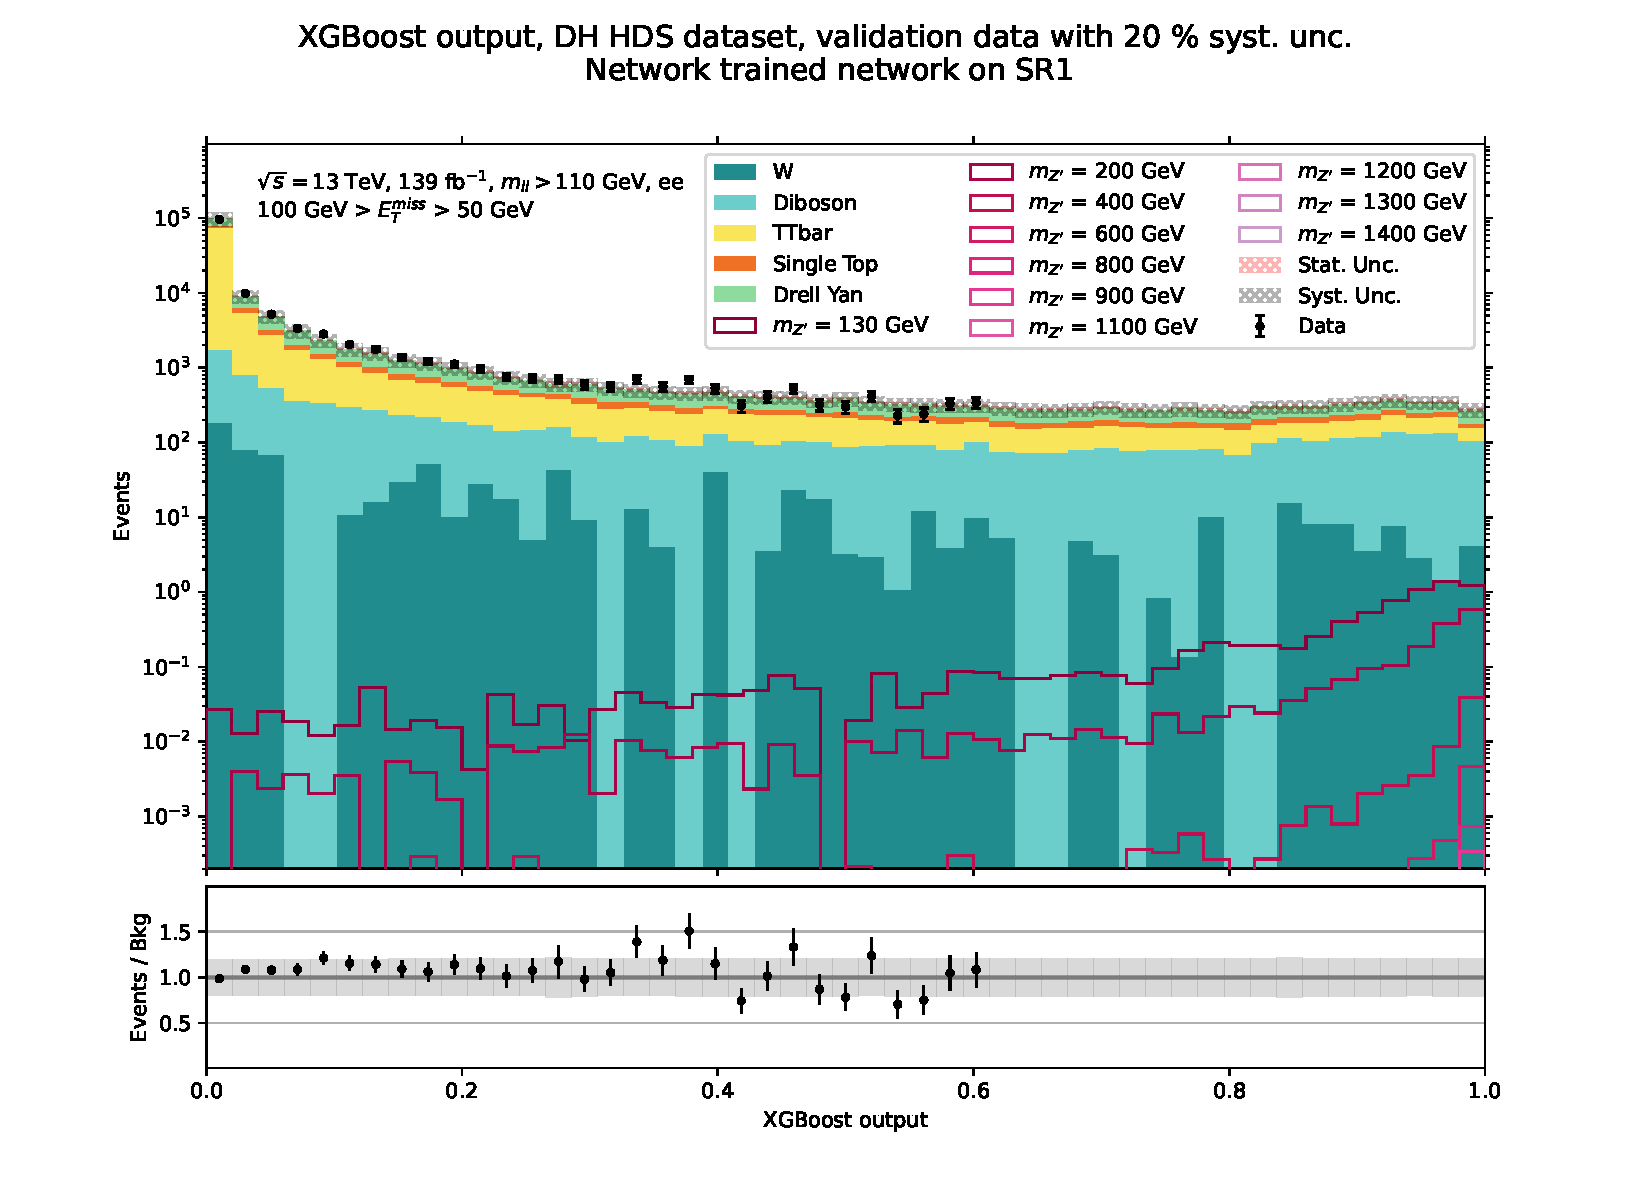
\includegraphics[width=1\textwidth]{XGBoost/Model_independent/50-100/DH_HDS/VAL_ee.pdf}
   \end{subfigure}
   \hfill
   \begin{subfigure}[b]{0.49\textwidth}
      \centering
      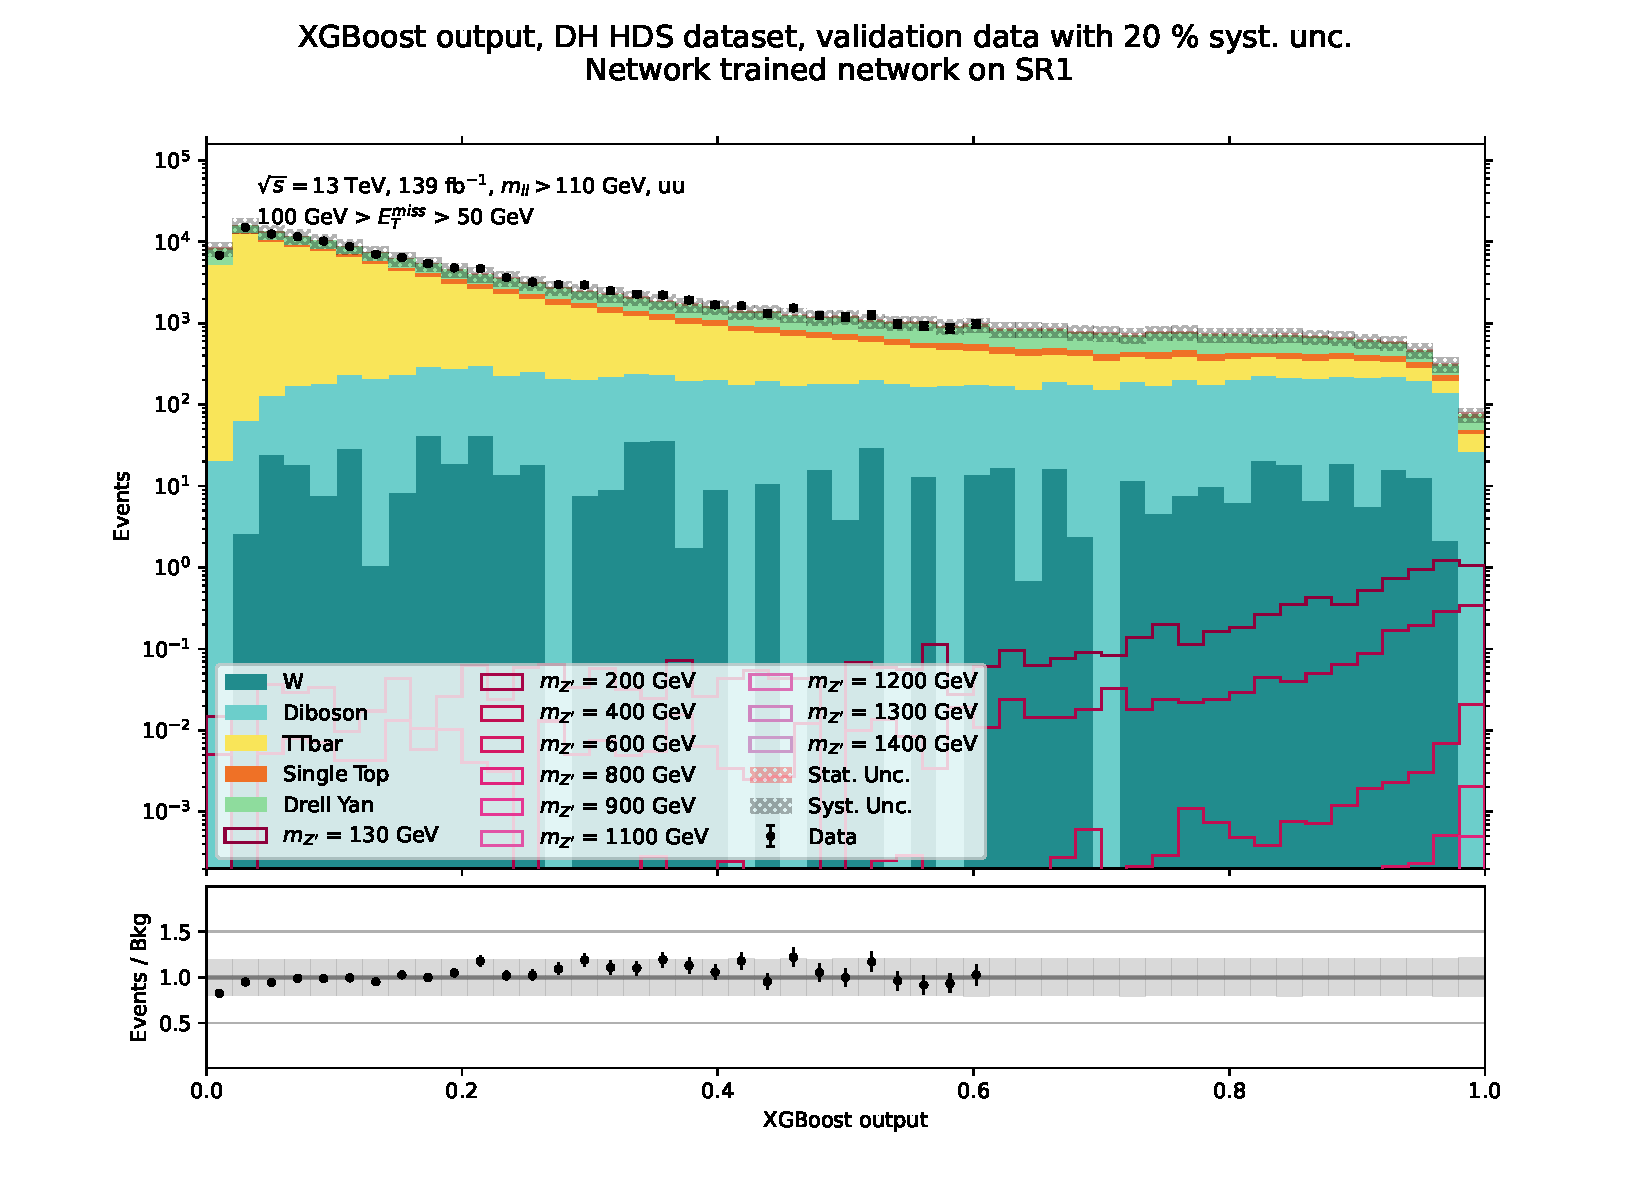
\includegraphics[width=1\textwidth]{XGBoost/Model_independent/50-100/DH_HDS/VAL_uu.pdf}
   \end{subfigure}
   \hfill
   \begin{subfigure}[b]{0.49\textwidth}
      \centering
      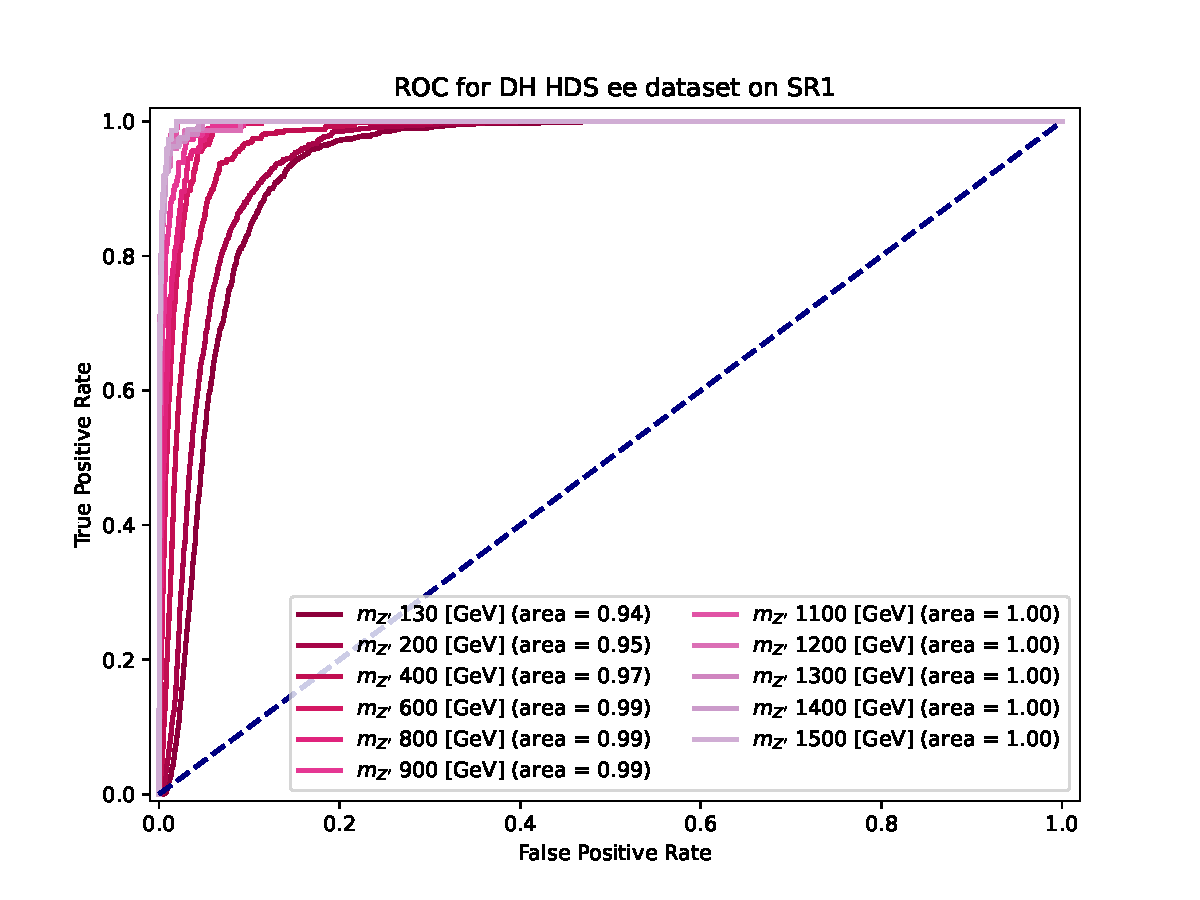
\includegraphics[width=1\textwidth]{XGBoost/Model_independent/50-100/DH_HDS/ROC_ee.pdf}
   \end{subfigure}
   \hfill
   \begin{subfigure}[b]{0.49\textwidth}
      \centering
      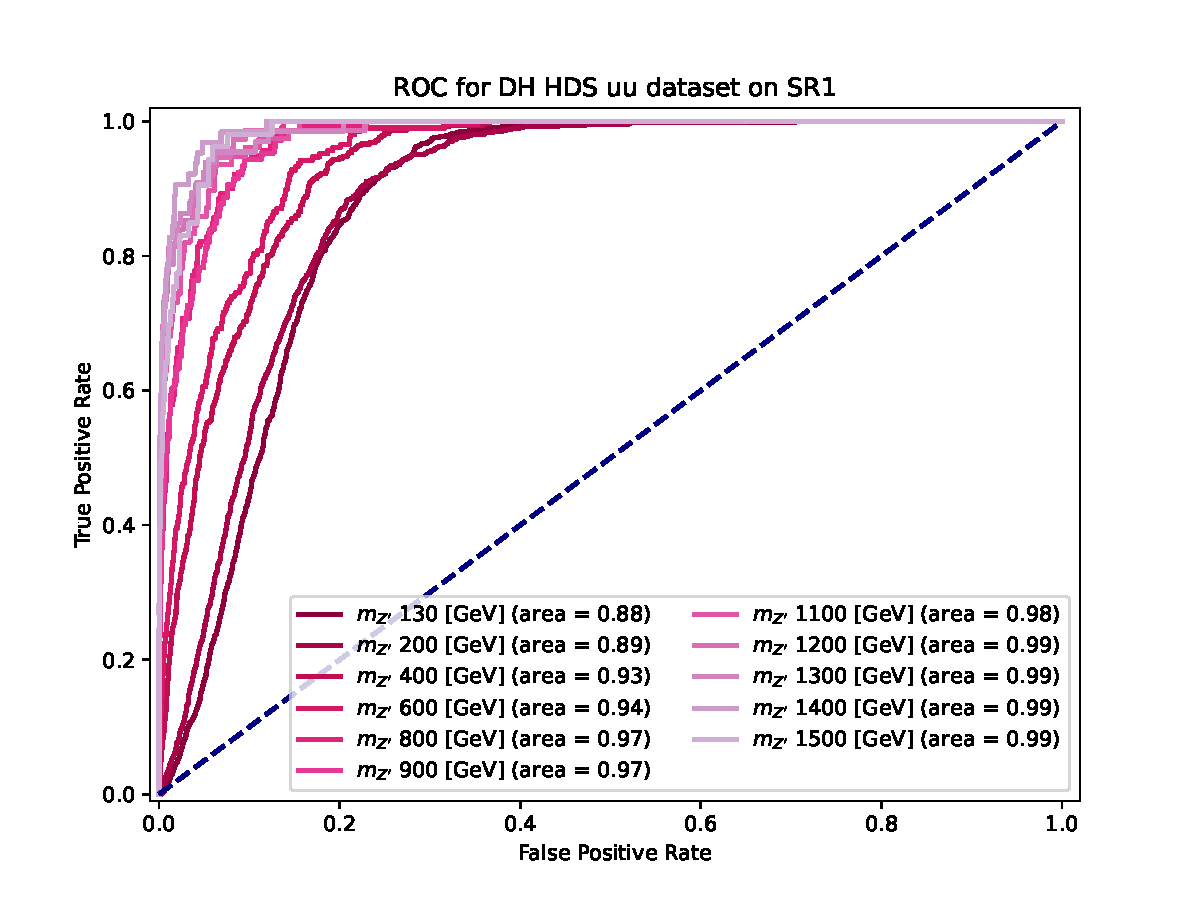
\includegraphics[width=1\textwidth]{XGBoost/Model_independent/50-100/DH_HDS/ROC_uu.pdf}
   \end{subfigure}
   \hfill
	\begin{subfigure}[b]{0.49\textwidth}
      \centering
      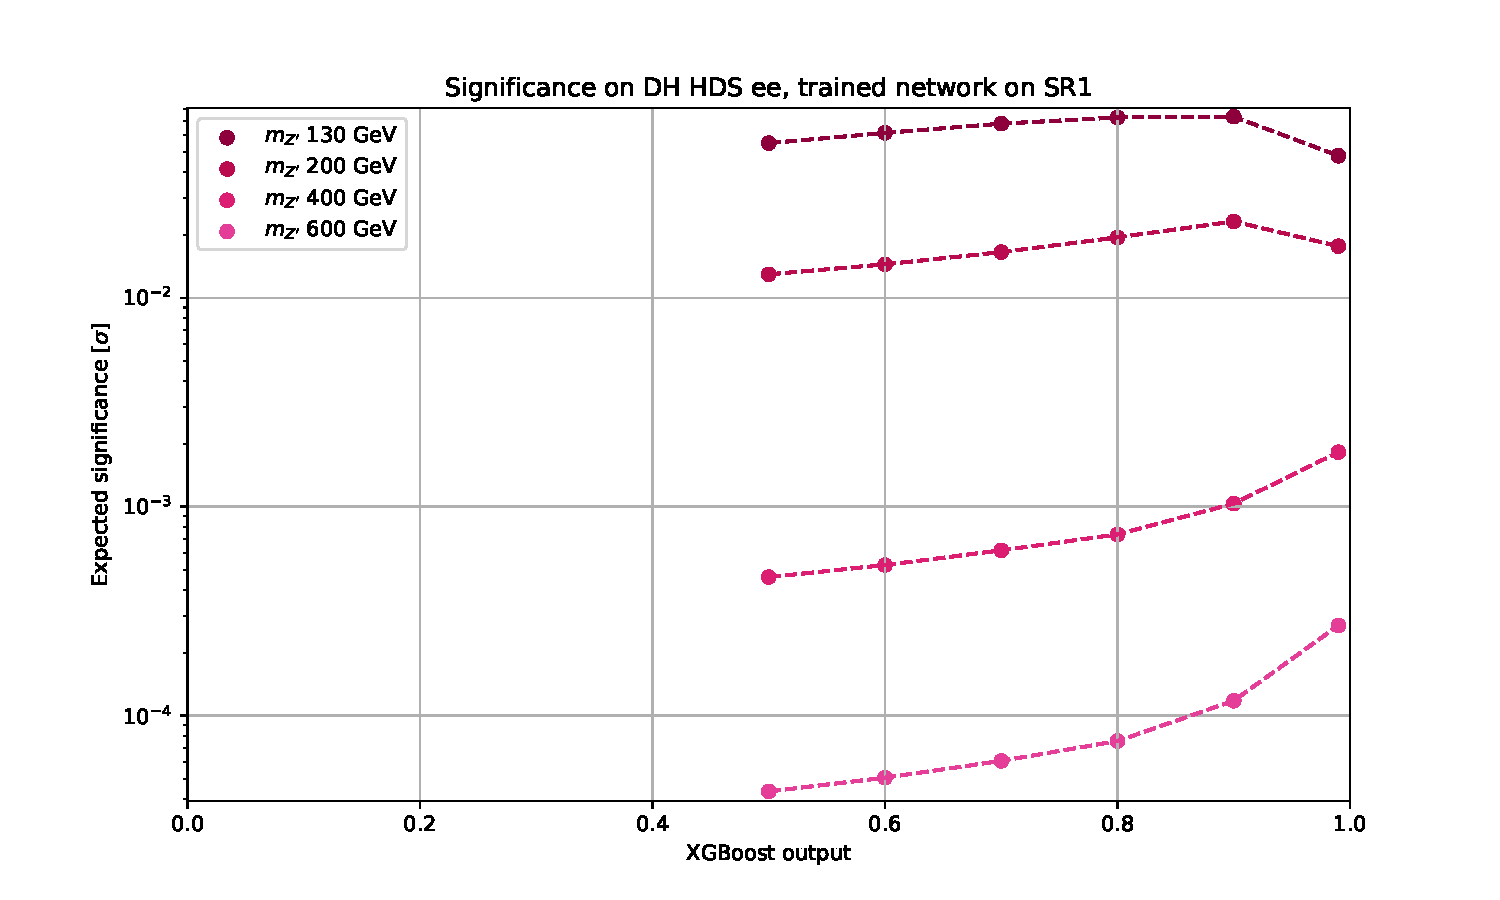
\includegraphics[width=1\textwidth]{XGBoost/Model_independent/50-100/DH_HDS/EXP_SIG_ee.pdf}
   \end{subfigure}
   \hfill
   \begin{subfigure}[b]{0.49\textwidth}
      \centering
      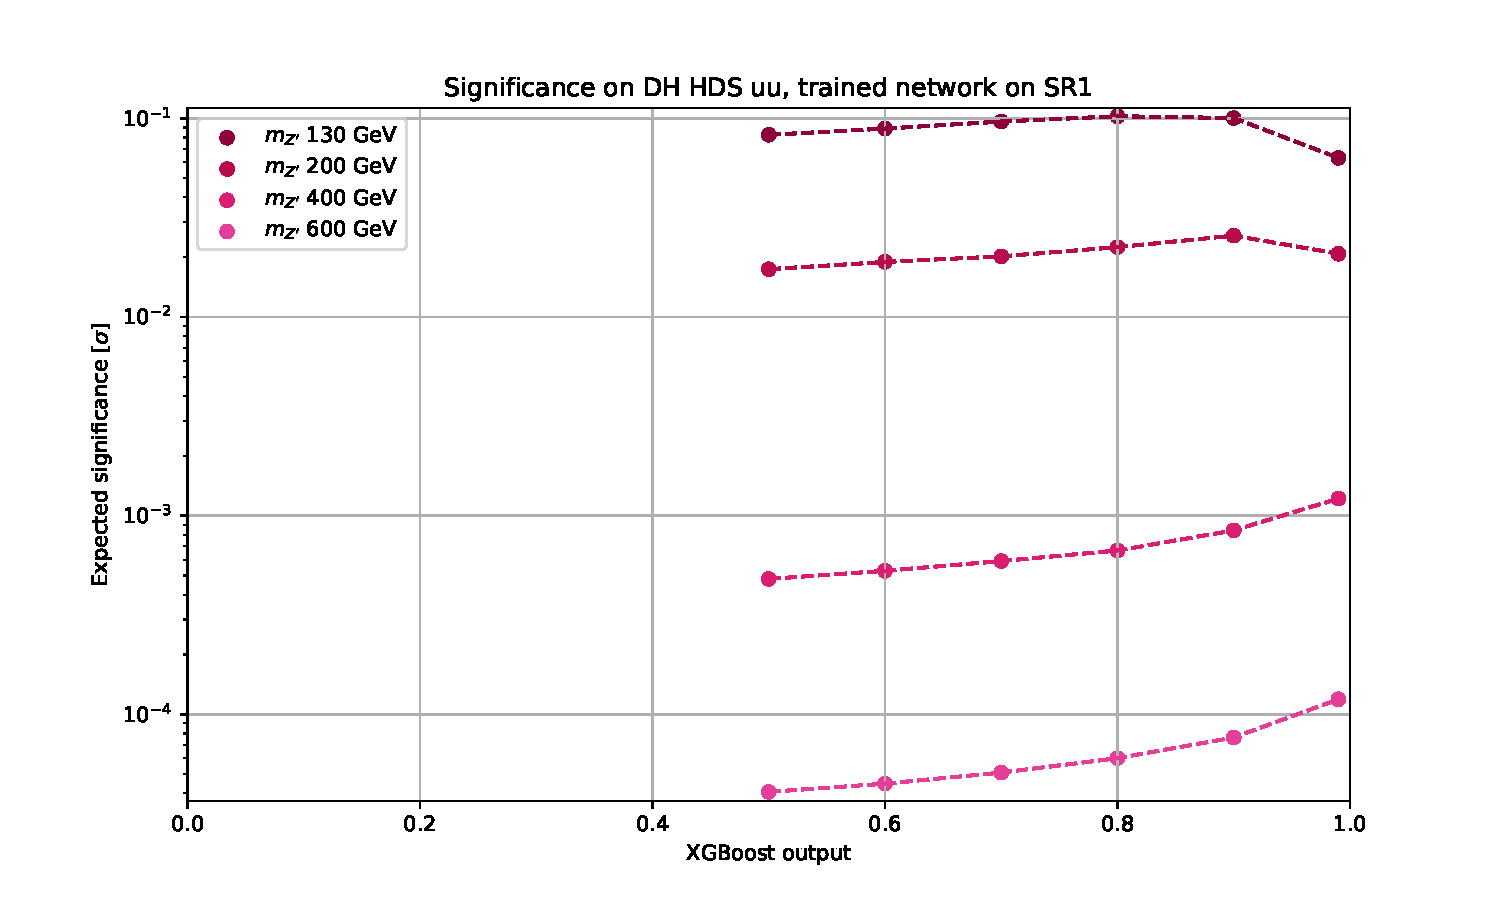
\includegraphics[width=1\textwidth]{XGBoost/Model_independent/50-100/DH_HDS/EXP_SIG_uu.pdf}
   \end{subfigure}
   \caption{XGBoost results for DH HDS model on $ee$ and $\mu\mu$ channel in SR1}\label{fig:DH_HDS_SR1}
\end{figure}

\begin{figure}[!ht]
	\centering
	\begin{subfigure}[b]{0.49\textwidth}
      \centering
      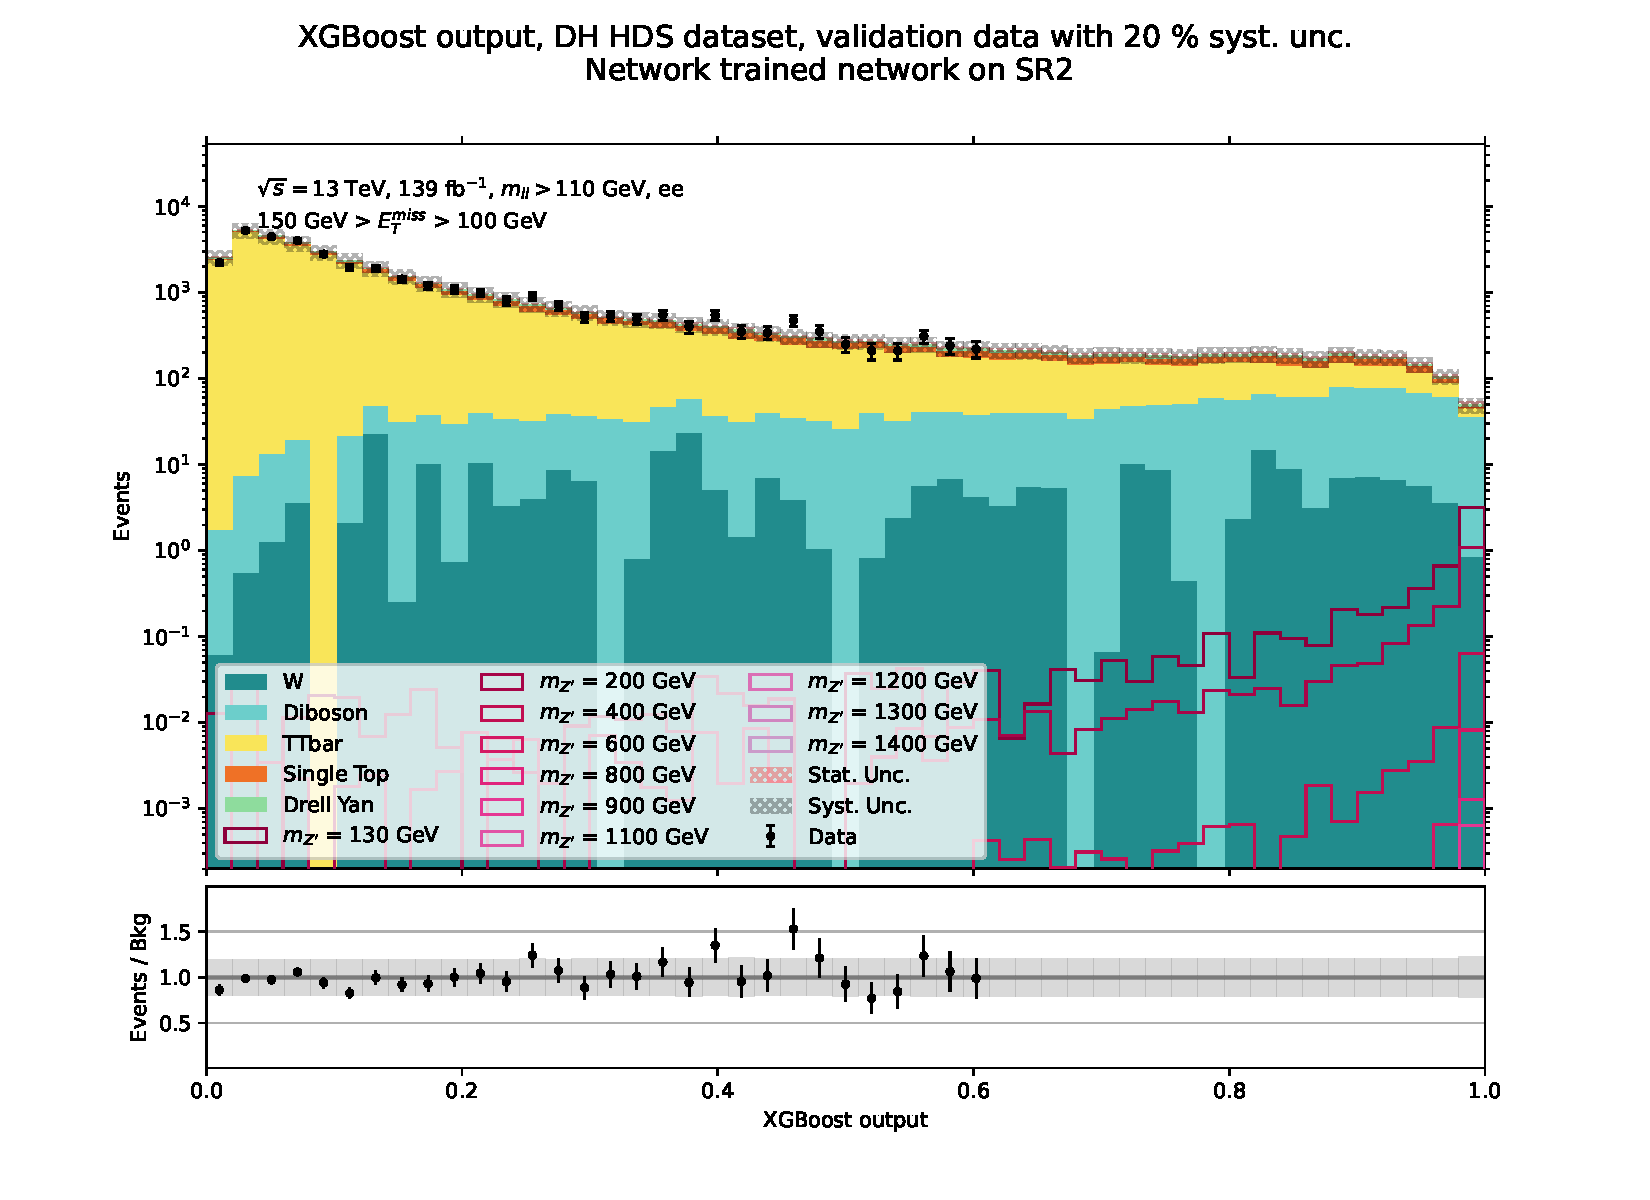
\includegraphics[width=1\textwidth]{XGBoost/Model_independent/100-150/DH_HDS/VAL_ee.pdf}
   \end{subfigure}
   \hfill
   \begin{subfigure}[b]{0.49\textwidth}
      \centering
      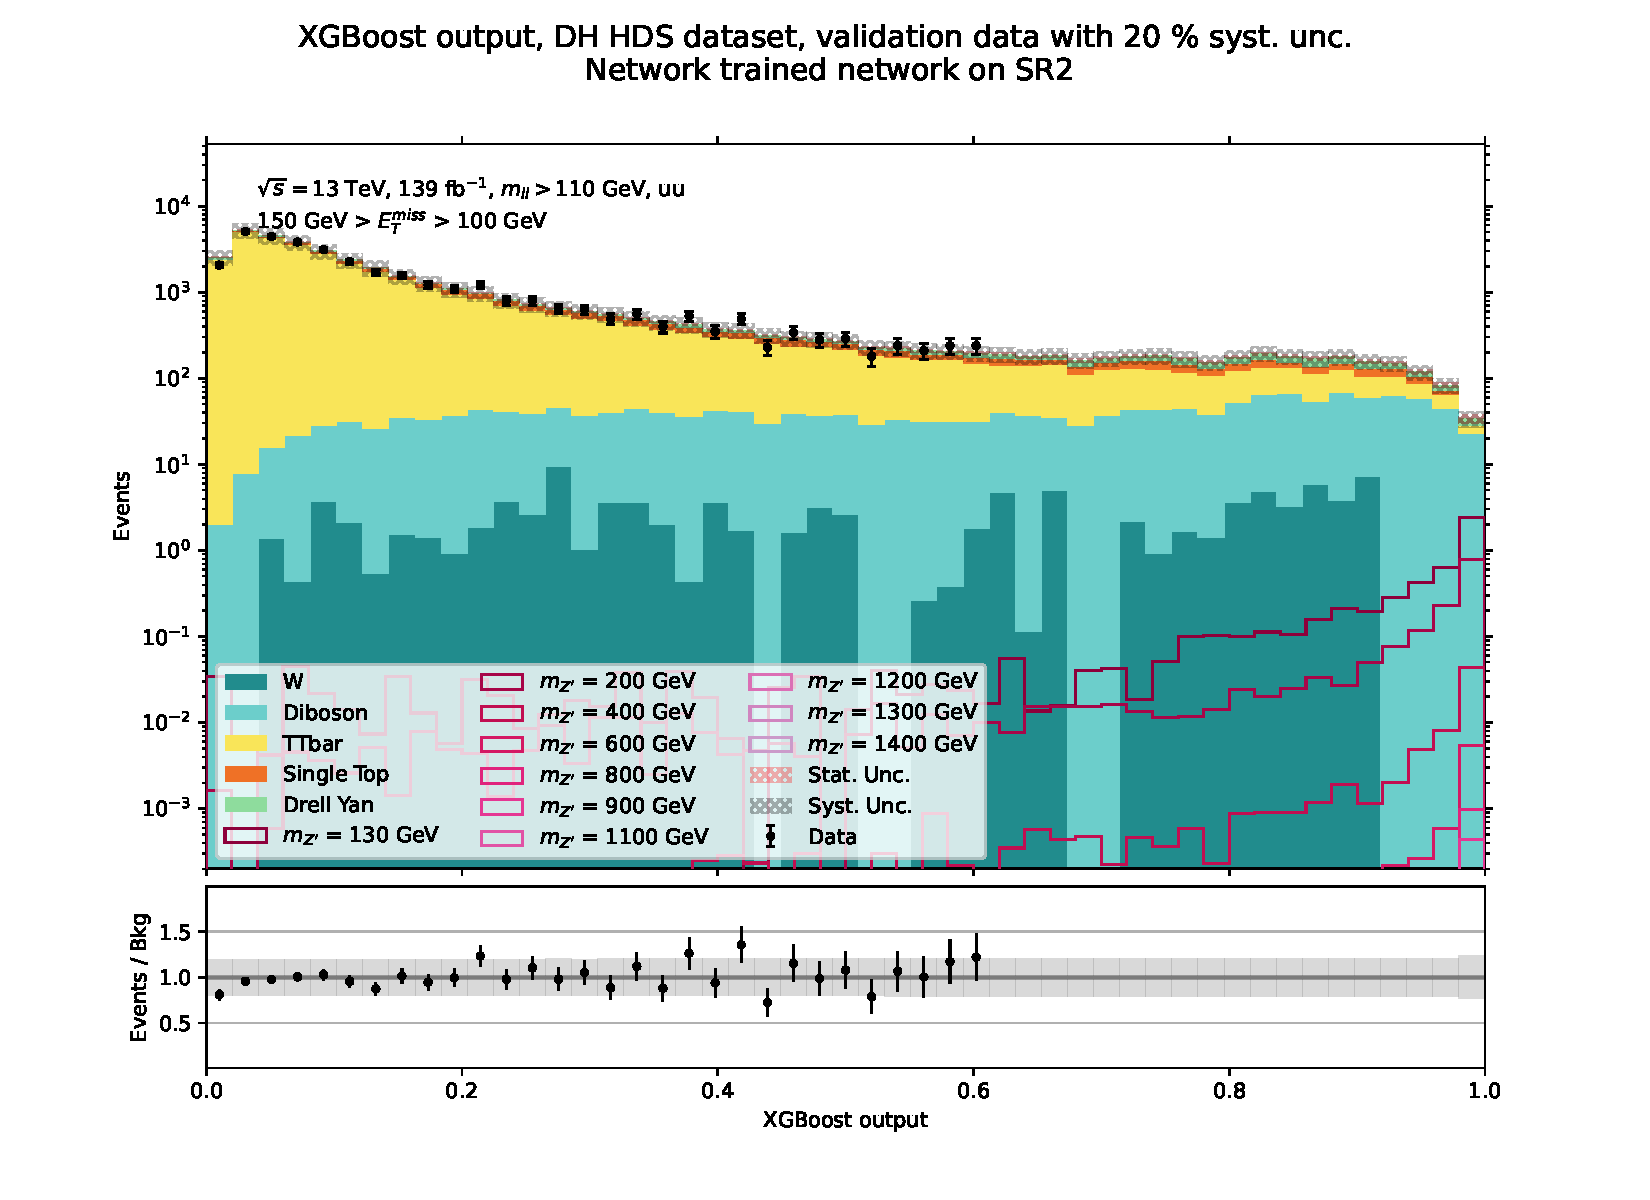
\includegraphics[width=1\textwidth]{XGBoost/Model_independent/100-150/DH_HDS/VAL_uu.pdf}
   \end{subfigure}
   \hfill
   \begin{subfigure}[b]{0.49\textwidth}
      \centering
      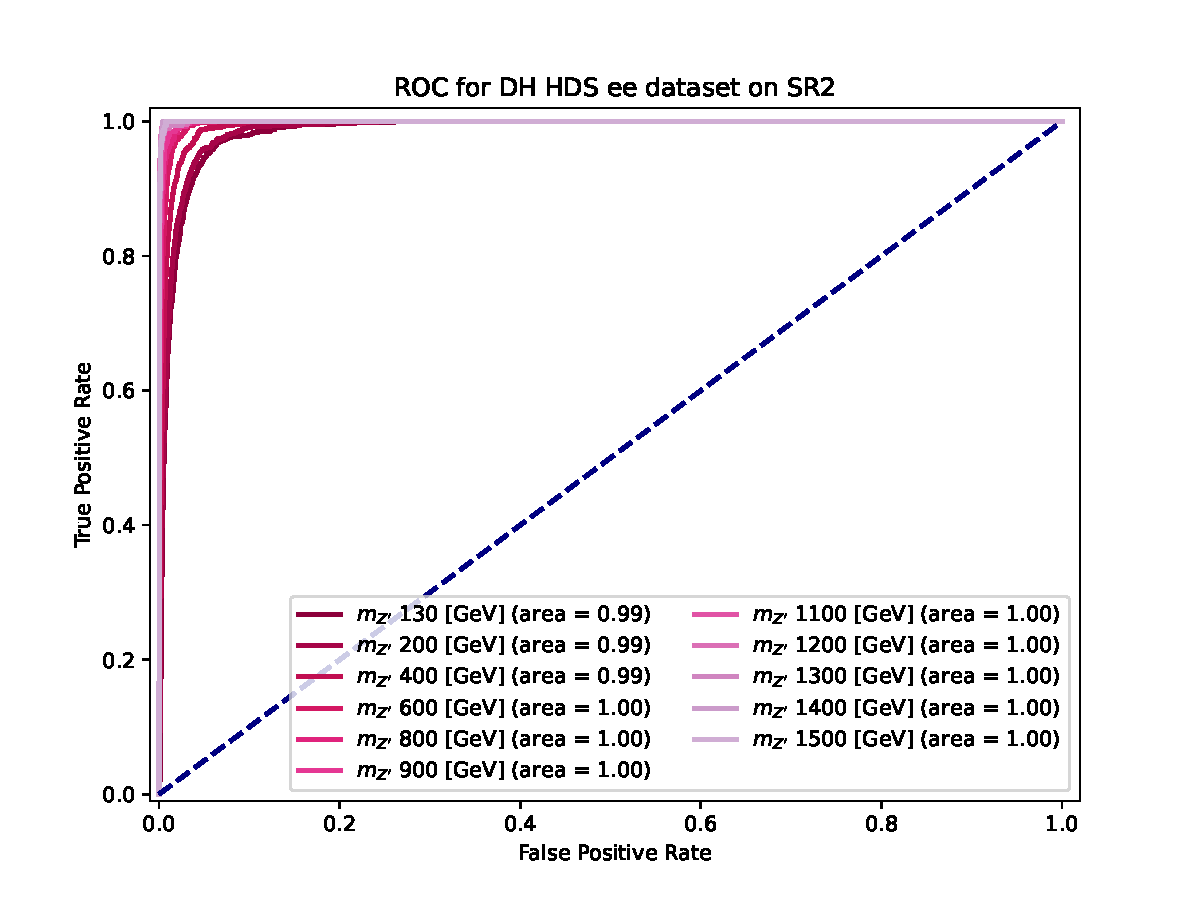
\includegraphics[width=1\textwidth]{XGBoost/Model_independent/100-150/DH_HDS/ROC_ee.pdf}
   \end{subfigure}
   \hfill
   \begin{subfigure}[b]{0.49\textwidth}
      \centering
      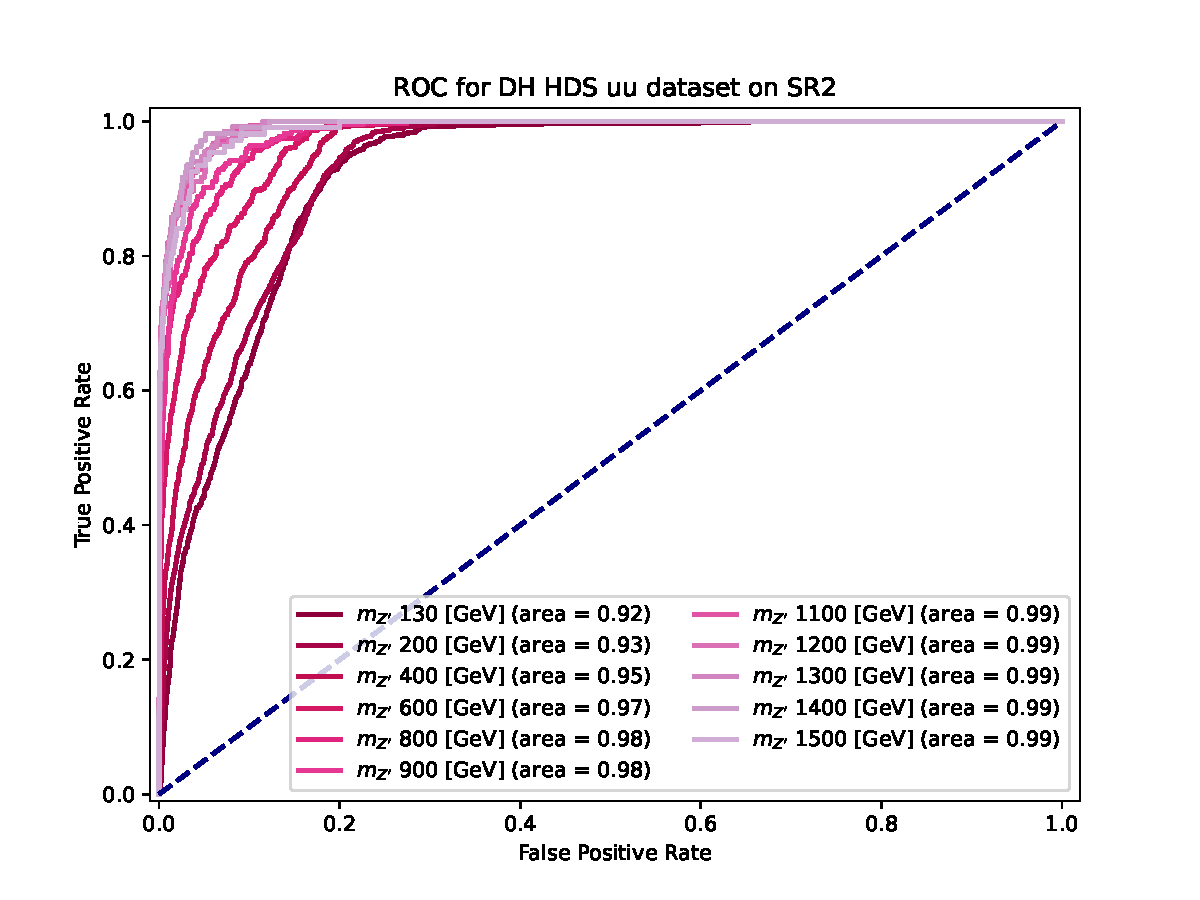
\includegraphics[width=1\textwidth]{XGBoost/Model_independent/100-150/DH_HDS/ROC_uu.pdf}
   \end{subfigure}
   \hfill
	\begin{subfigure}[b]{0.49\textwidth}
      \centering
      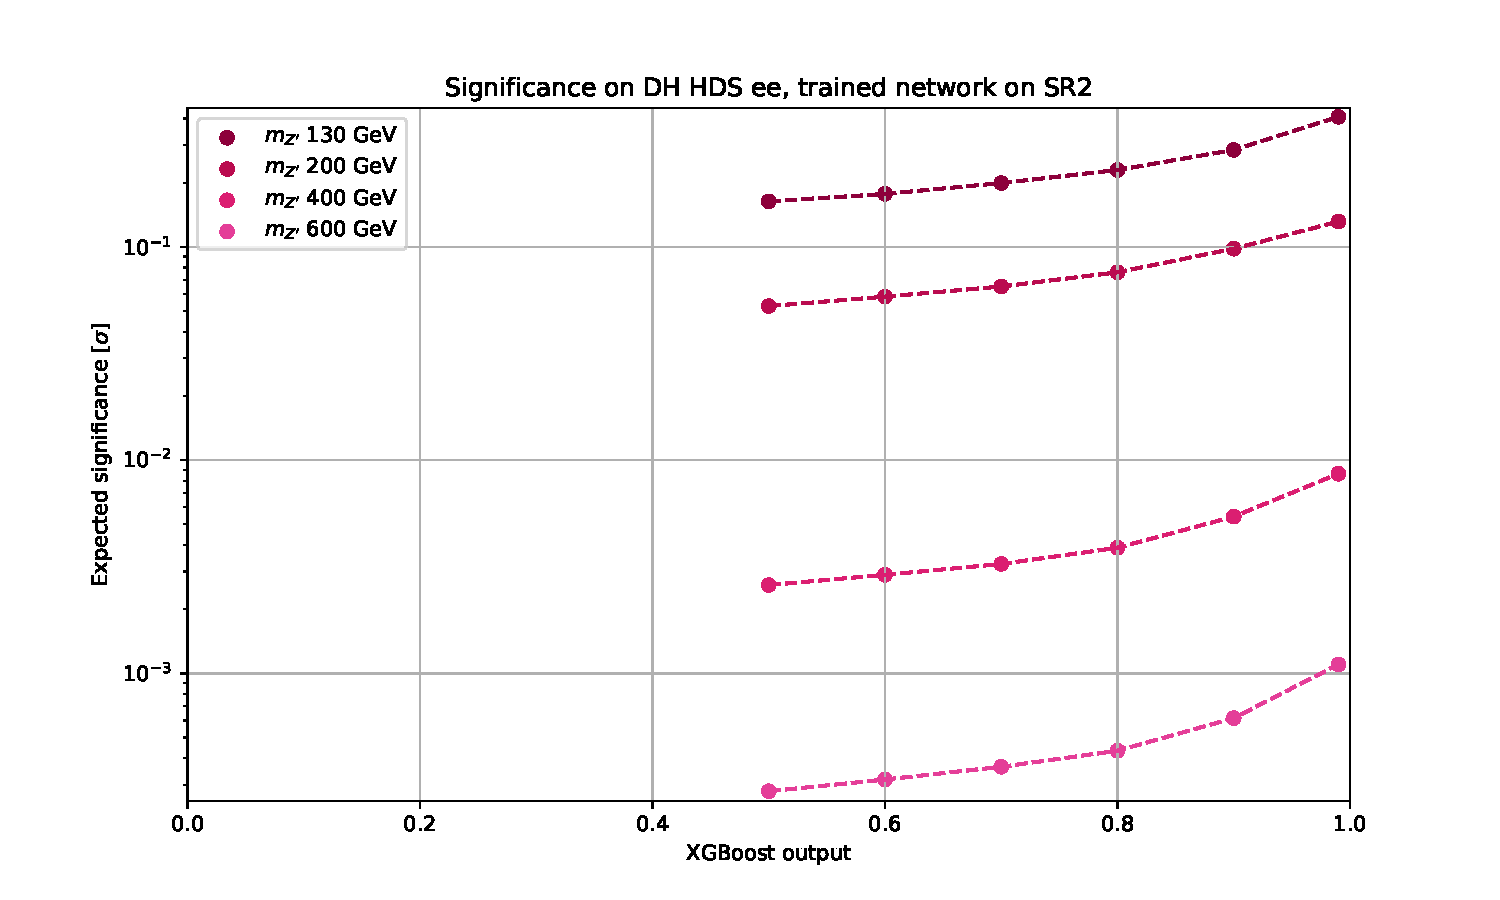
\includegraphics[width=1\textwidth]{XGBoost/Model_independent/100-150/DH_HDS/EXP_SIG_ee.pdf}
   \end{subfigure}
   \hfill
   \begin{subfigure}[b]{0.49\textwidth}
      \centering
      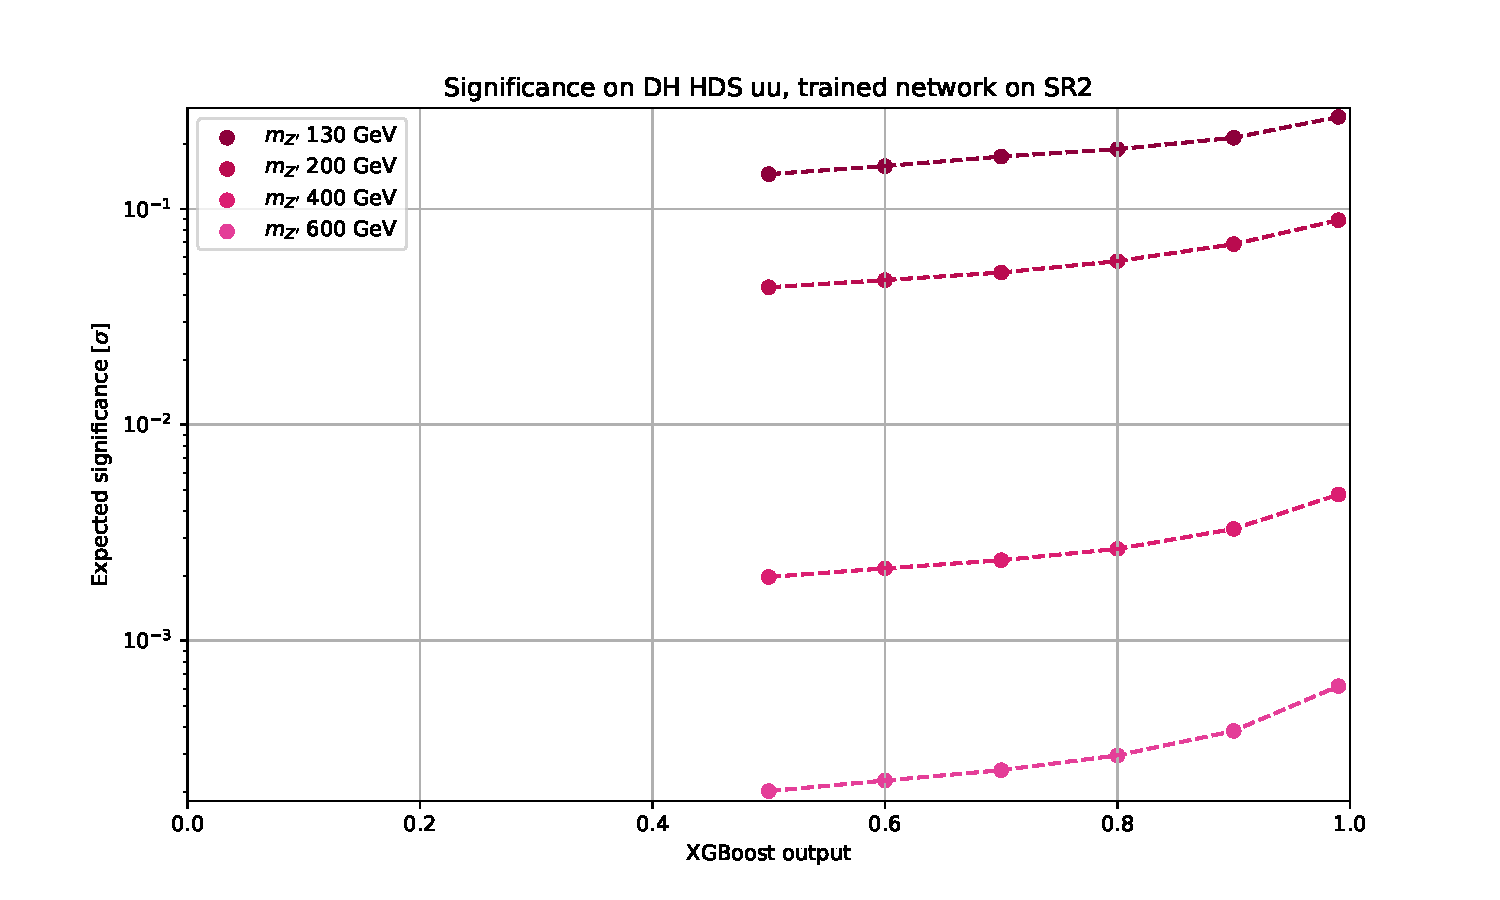
\includegraphics[width=1\textwidth]{XGBoost/Model_independent/100-150/DH_HDS/EXP_SIG_uu.pdf}
   \end{subfigure}
   \caption{XGBoost results for DH HDS model on $ee$ and $\mu\mu$ channel in SR2}\label{fig:DH_HDS_SR2}
\end{figure}

\begin{figure}[!ht]
	\centering
	\begin{subfigure}[b]{0.49\textwidth}
      \centering
      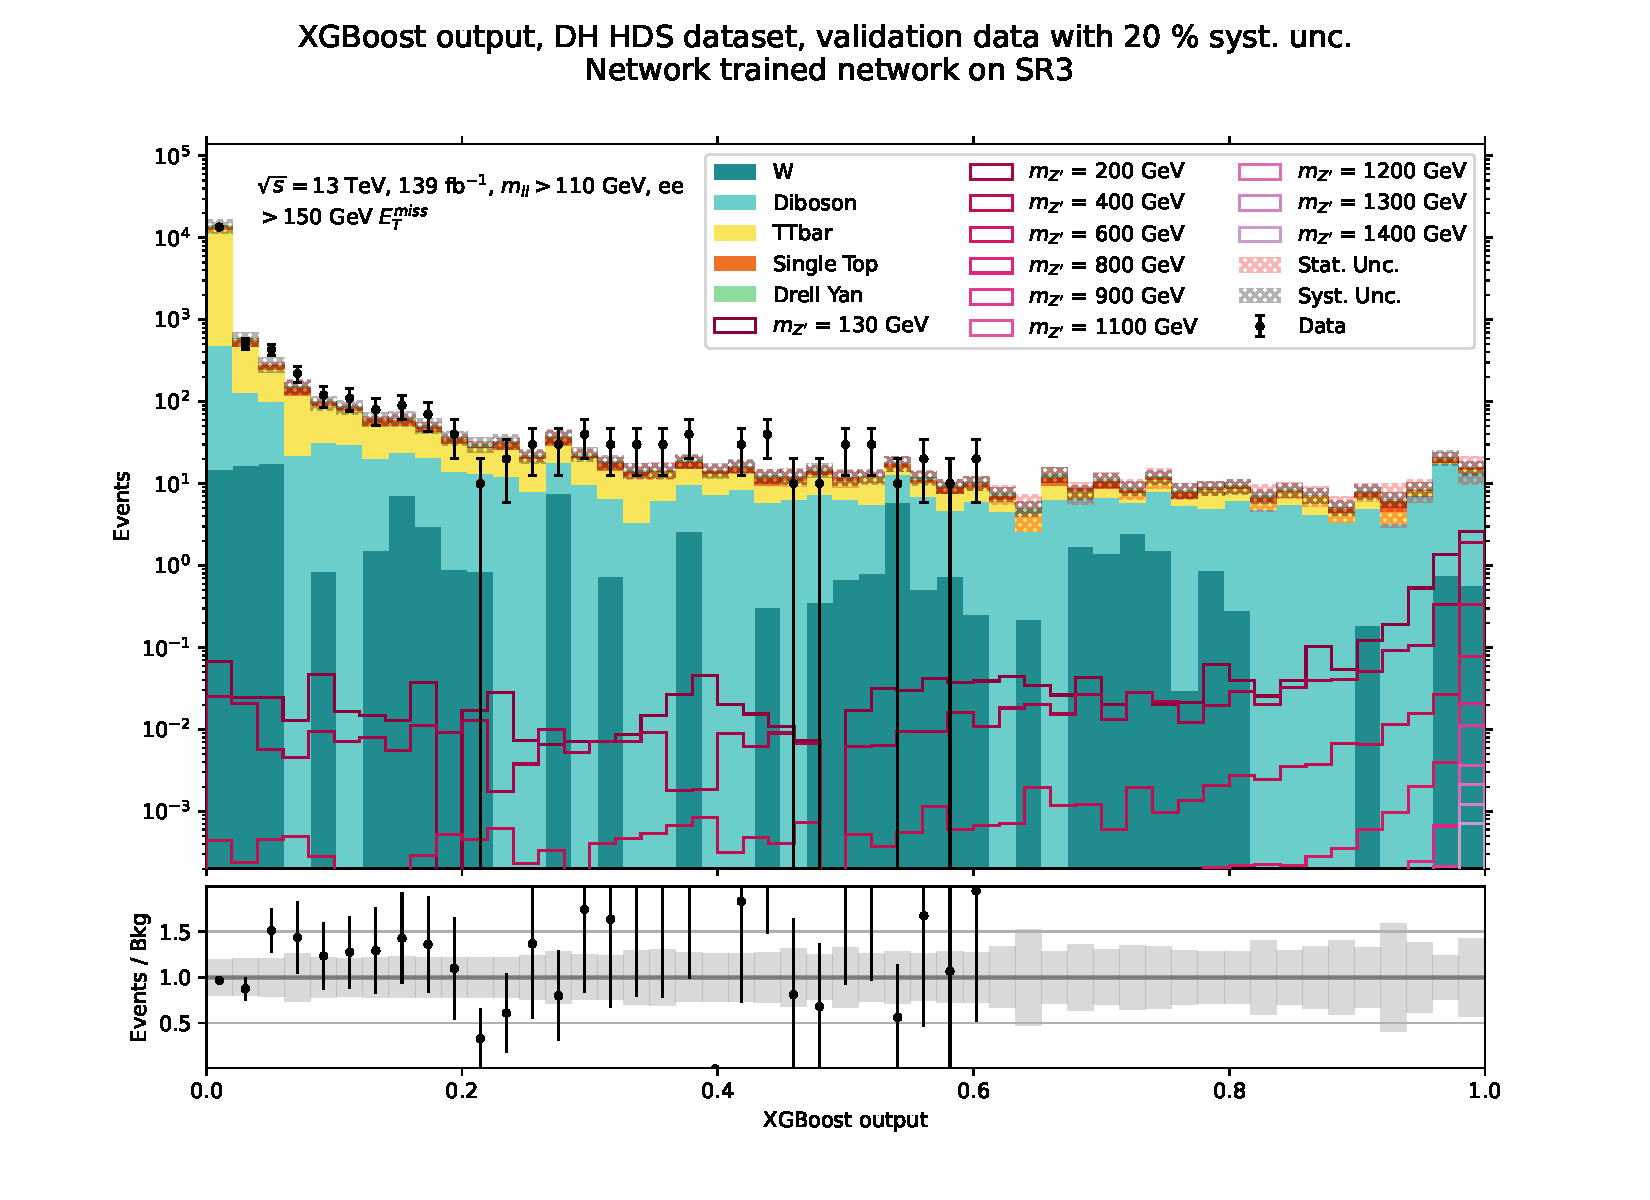
\includegraphics[width=1\textwidth]{XGBoost/Model_independent/150/DH_HDS/VAL_ee.pdf}
   \end{subfigure}
   \hfill
   \begin{subfigure}[b]{0.49\textwidth}
      \centering
      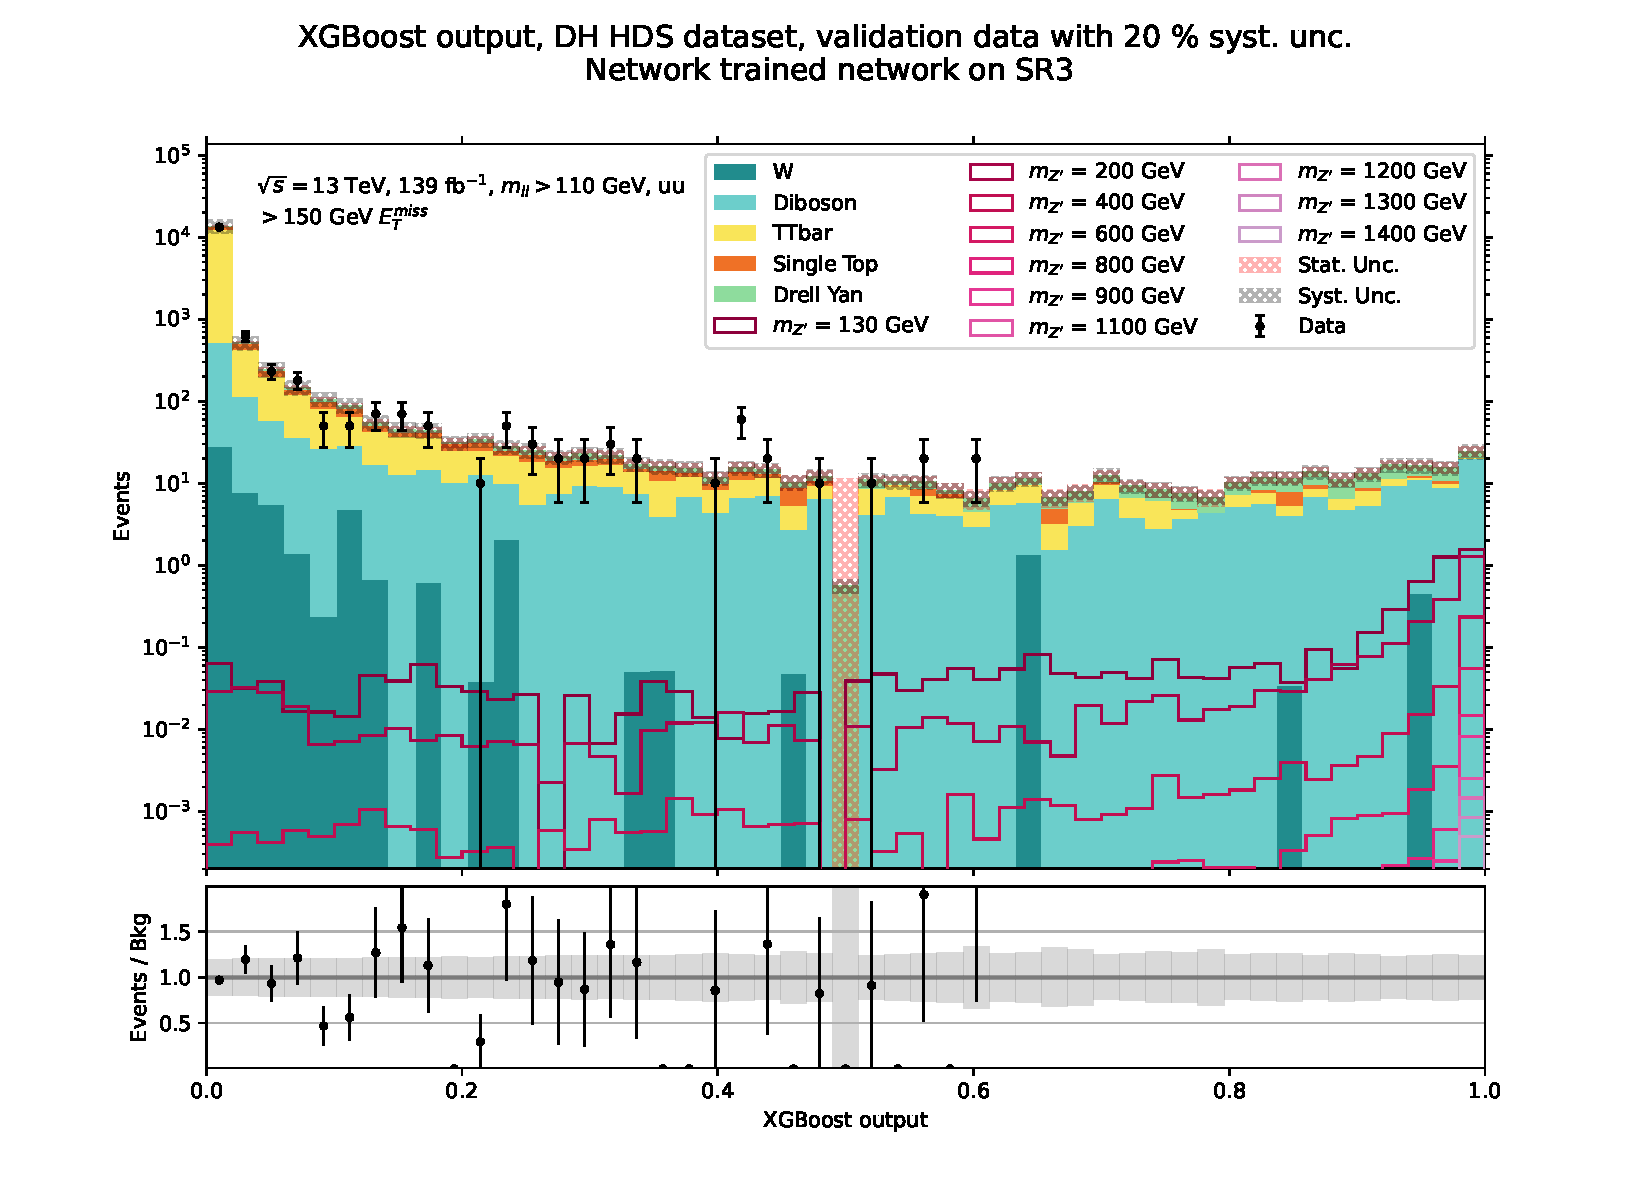
\includegraphics[width=1\textwidth]{XGBoost/Model_independent/150/DH_HDS/VAL_uu.pdf}
   \end{subfigure}
   \hfill
   \begin{subfigure}[b]{0.49\textwidth}
      \centering
      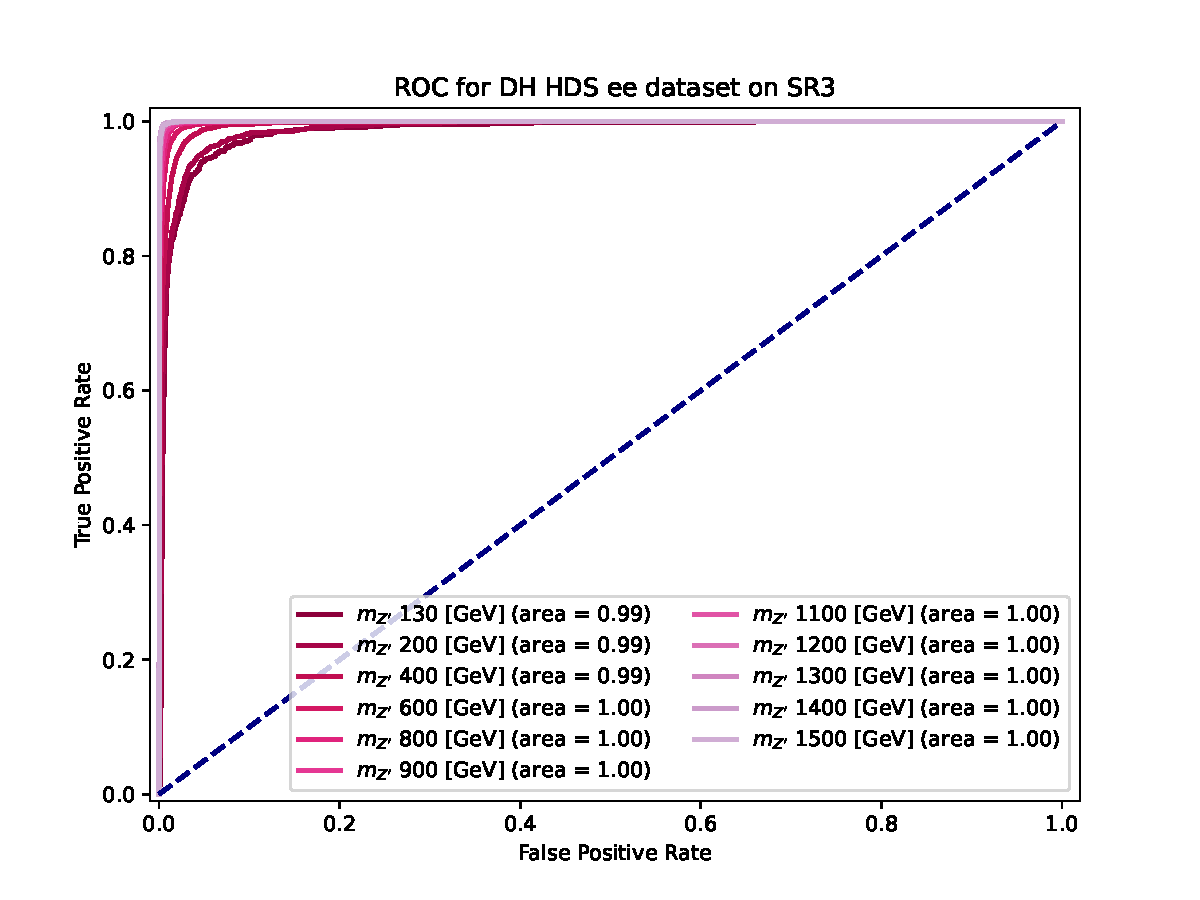
\includegraphics[width=1\textwidth]{XGBoost/Model_independent/150/DH_HDS/ROC_ee.pdf}
   \end{subfigure}
   \hfill
   \begin{subfigure}[b]{0.49\textwidth}
      \centering
      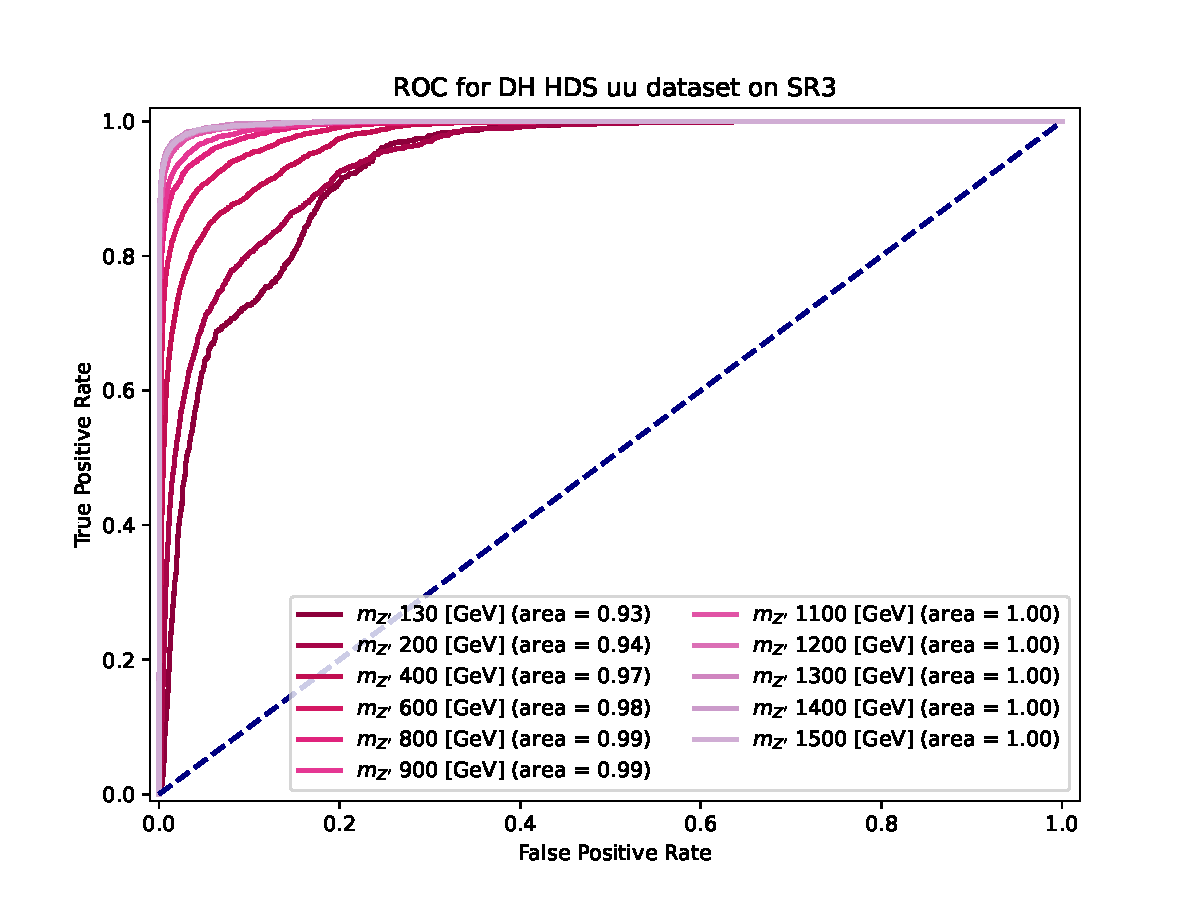
\includegraphics[width=1\textwidth]{XGBoost/Model_independent/150/DH_HDS/ROC_uu.pdf}
   \end{subfigure}
   \hfill
	\begin{subfigure}[b]{0.49\textwidth}
      \centering
      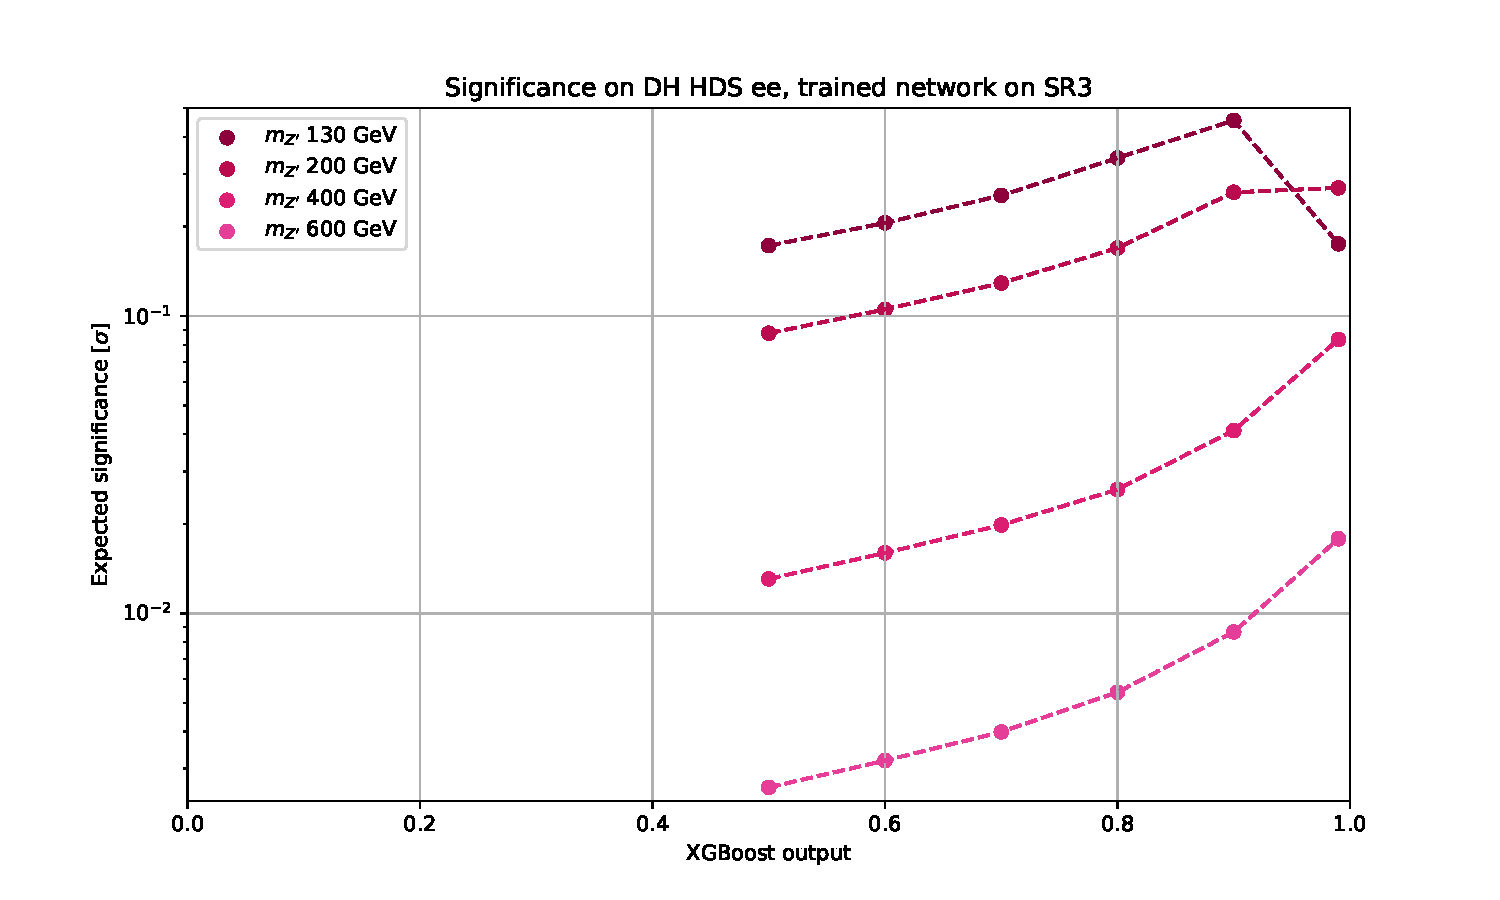
\includegraphics[width=1\textwidth]{XGBoost/Model_independent/150/DH_HDS/EXP_SIG_ee.pdf}
   \end{subfigure}
   \hfill
   \begin{subfigure}[b]{0.49\textwidth}
      \centering
      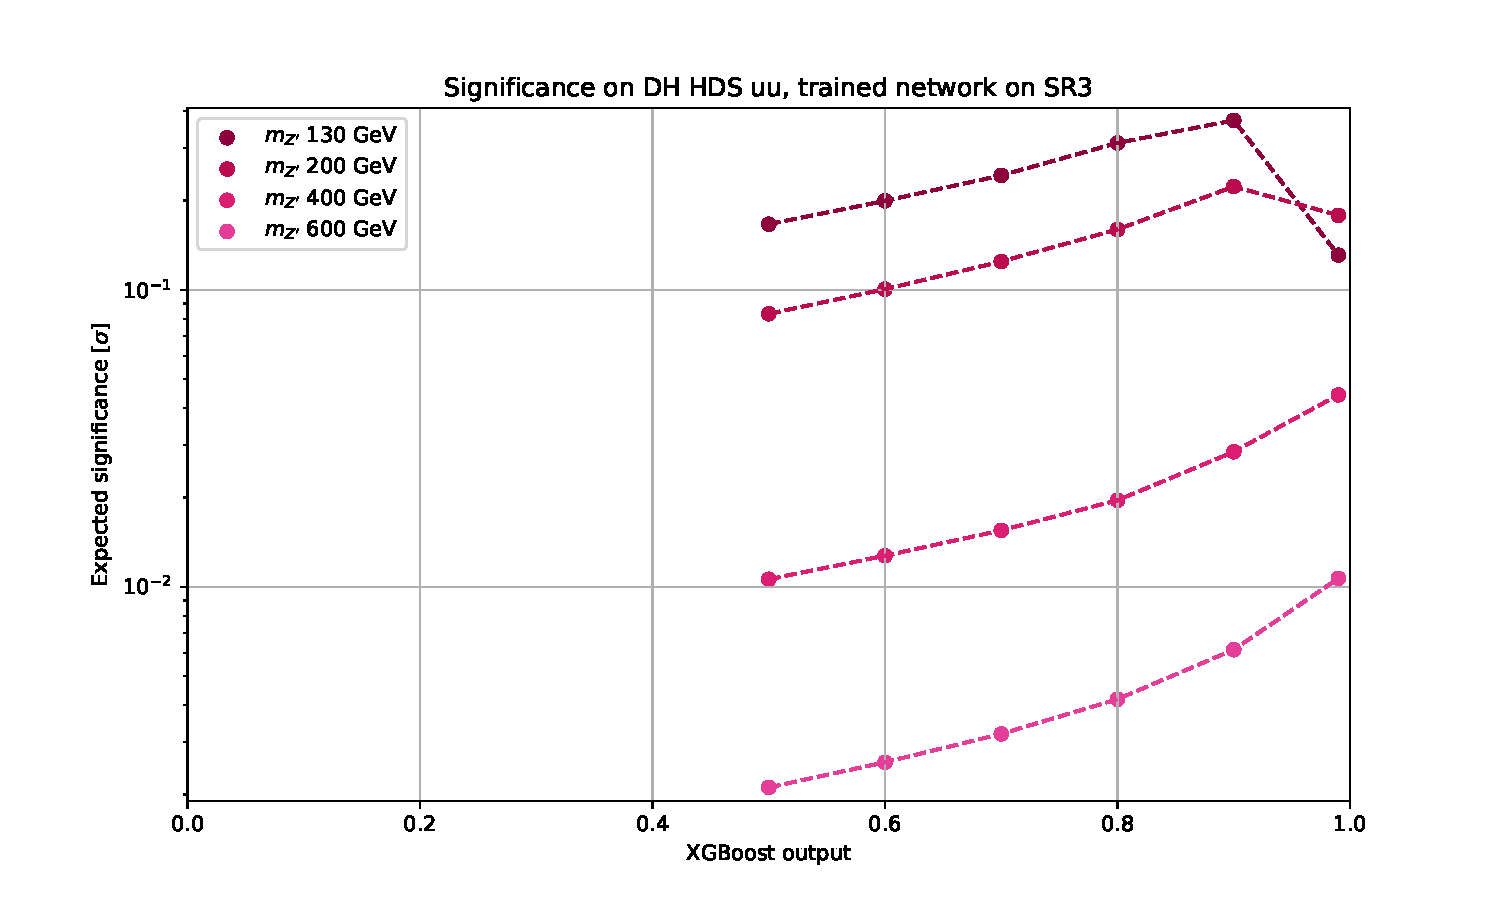
\includegraphics[width=1\textwidth]{XGBoost/Model_independent/150/DH_HDS/EXP_SIG_uu.pdf}
   \end{subfigure}
   \caption{XGBoost results for DH HDS model on $ee$ and $\mu\mu$ channel in SR3}\label{fig:DH_HDS_SR3}
\end{figure}

\begin{figure}[!ht]
	\centering
	\begin{subfigure}[b]{0.49\textwidth}
      \centering
      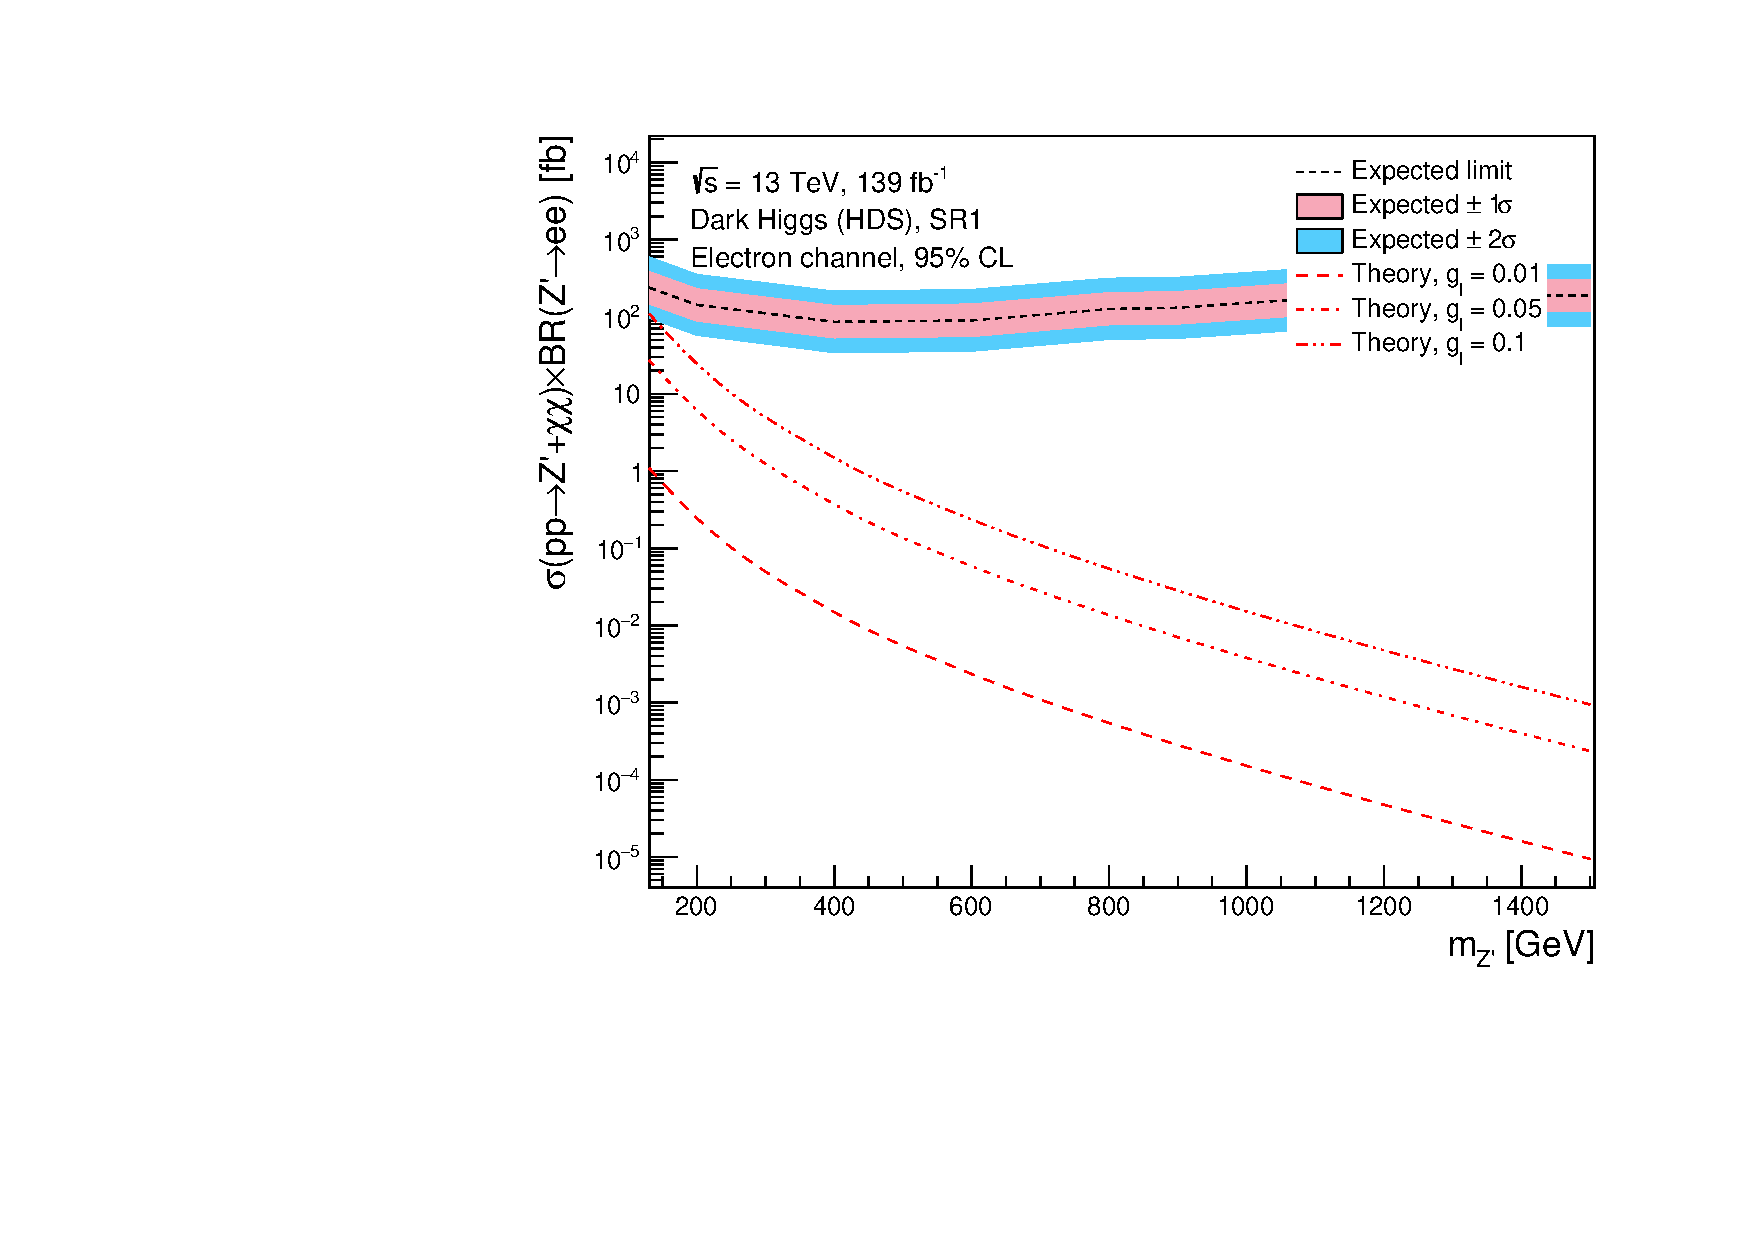
\includegraphics[width=1\textwidth]{Limits/Model_independent/50-100/DH_HDS/mass_exclusion_ee.pdf}
   \end{subfigure}
   \hfill
   \begin{subfigure}[b]{0.49\textwidth}
      \centering
      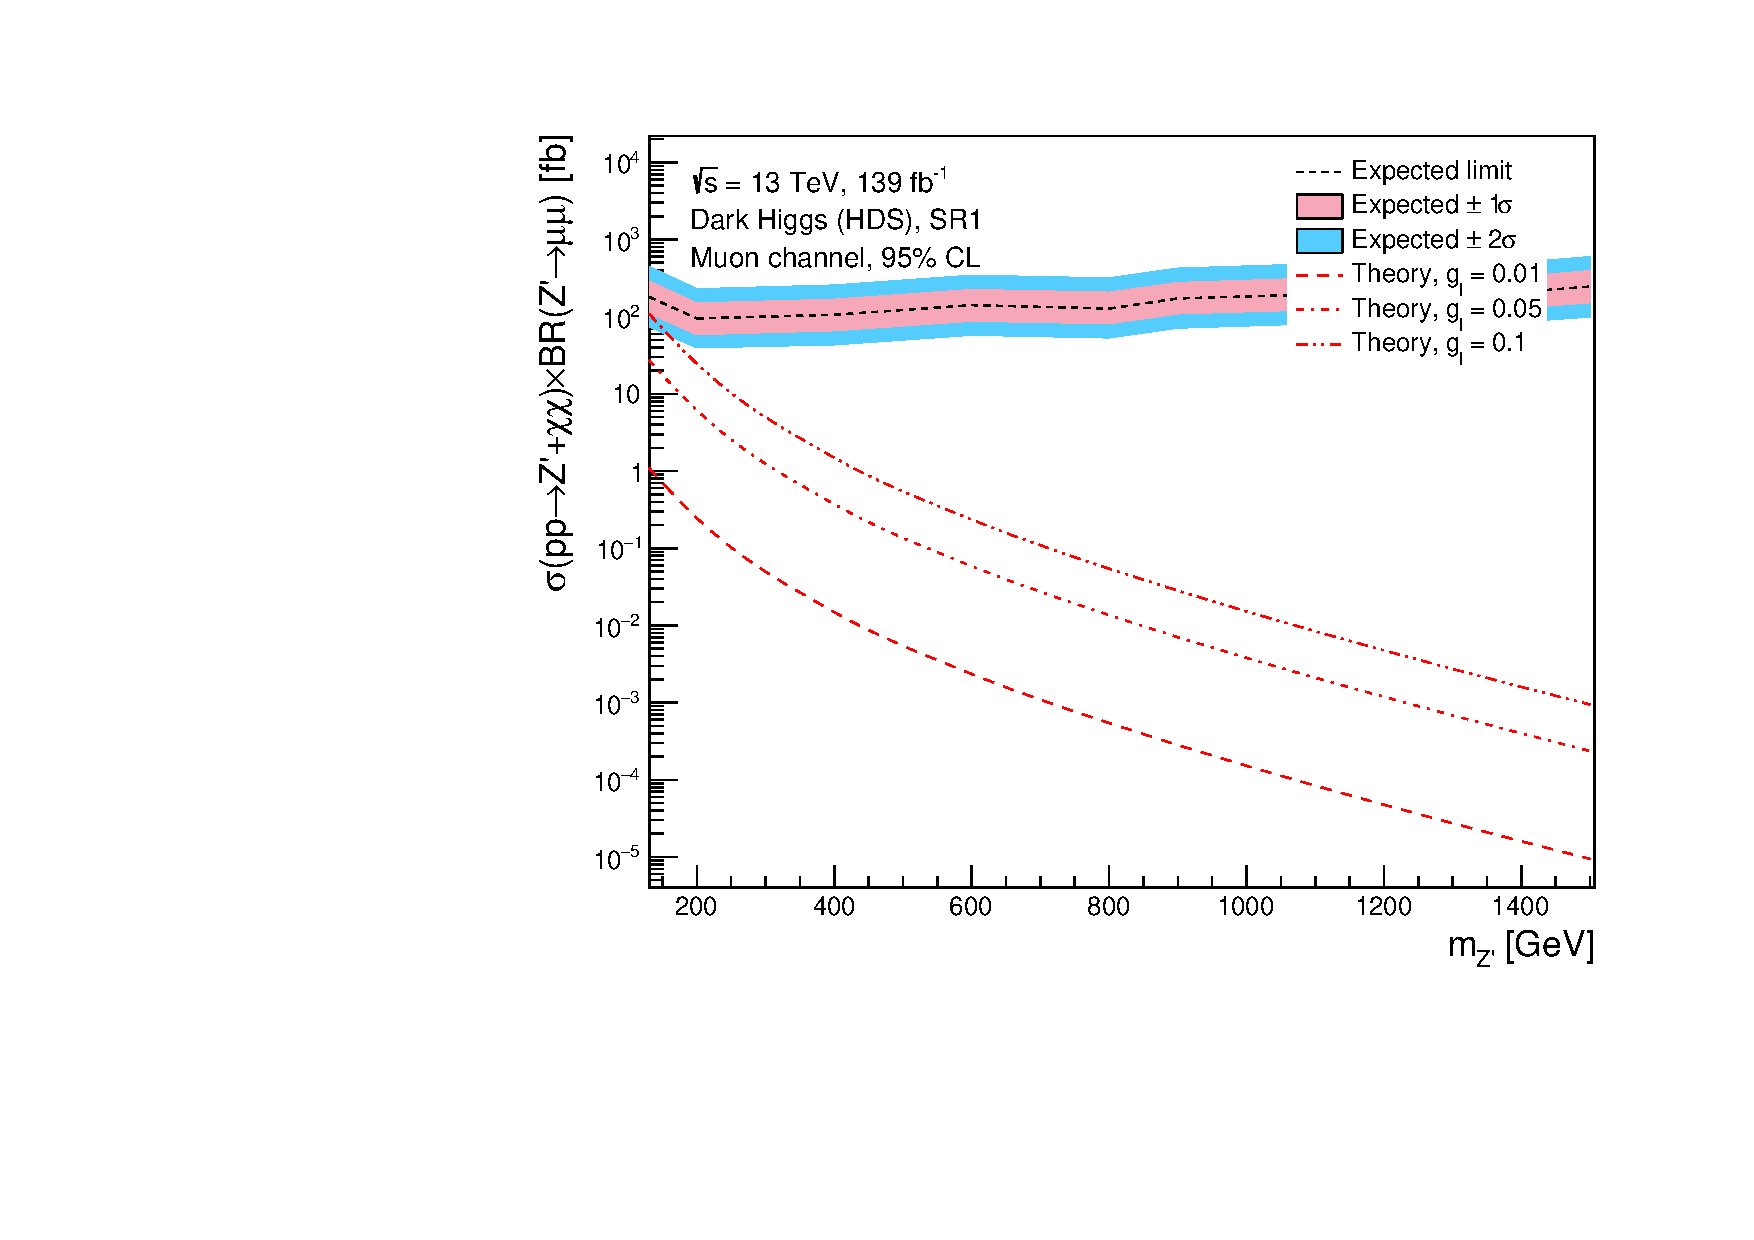
\includegraphics[width=1\textwidth]{Limits/Model_independent/50-100/DH_HDS/mass_exclusion_uu.pdf}
   \end{subfigure}
   \hfill
   \begin{subfigure}[b]{0.49\textwidth}
      \centering
      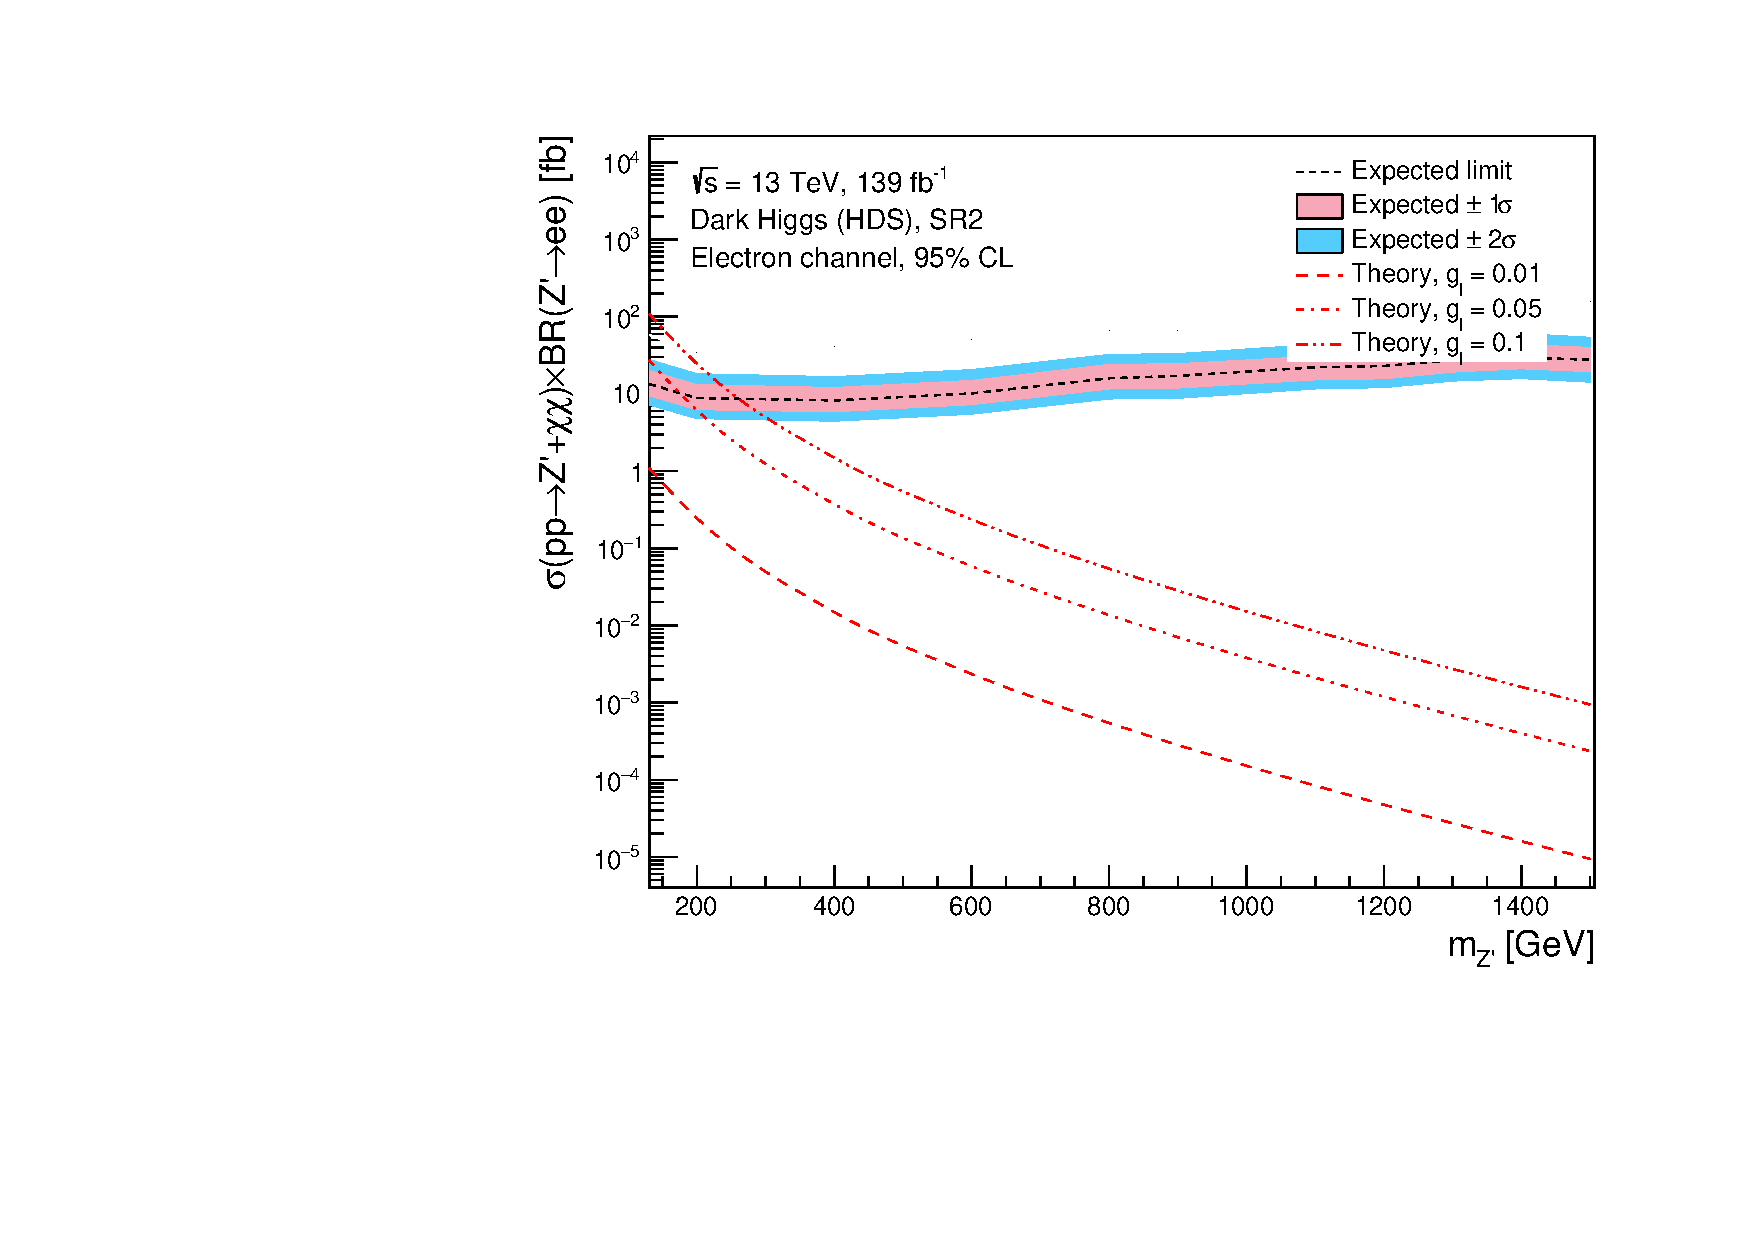
\includegraphics[width=1\textwidth]{Limits/Model_independent/100-150/DH_HDS/mass_exclusion_ee.pdf}
   \end{subfigure}
   \hfill
   \begin{subfigure}[b]{0.49\textwidth}
      \centering
      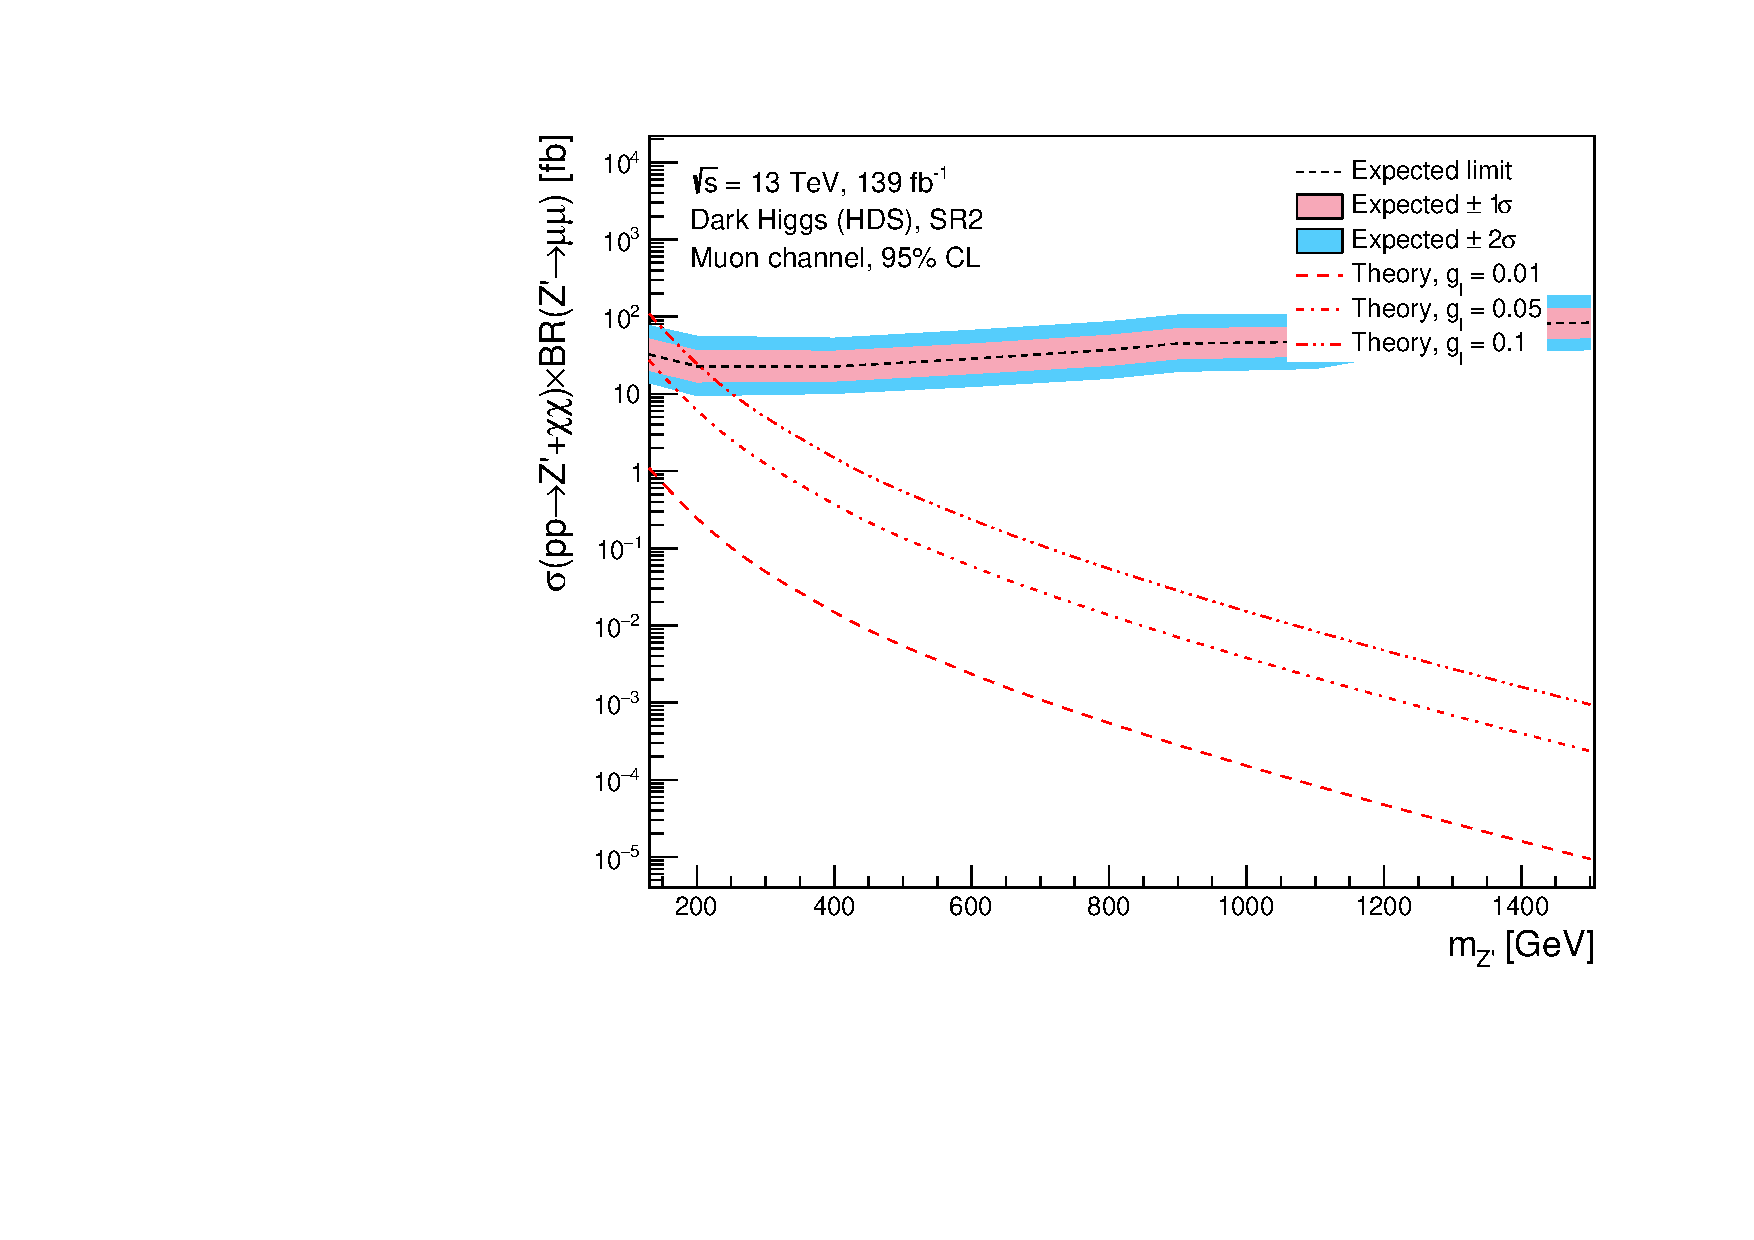
\includegraphics[width=1\textwidth]{Limits/Model_independent/100-150/DH_HDS/mass_exclusion_uu.pdf}
   \end{subfigure}
   \hfill
	\begin{subfigure}[b]{0.49\textwidth}
      \centering
      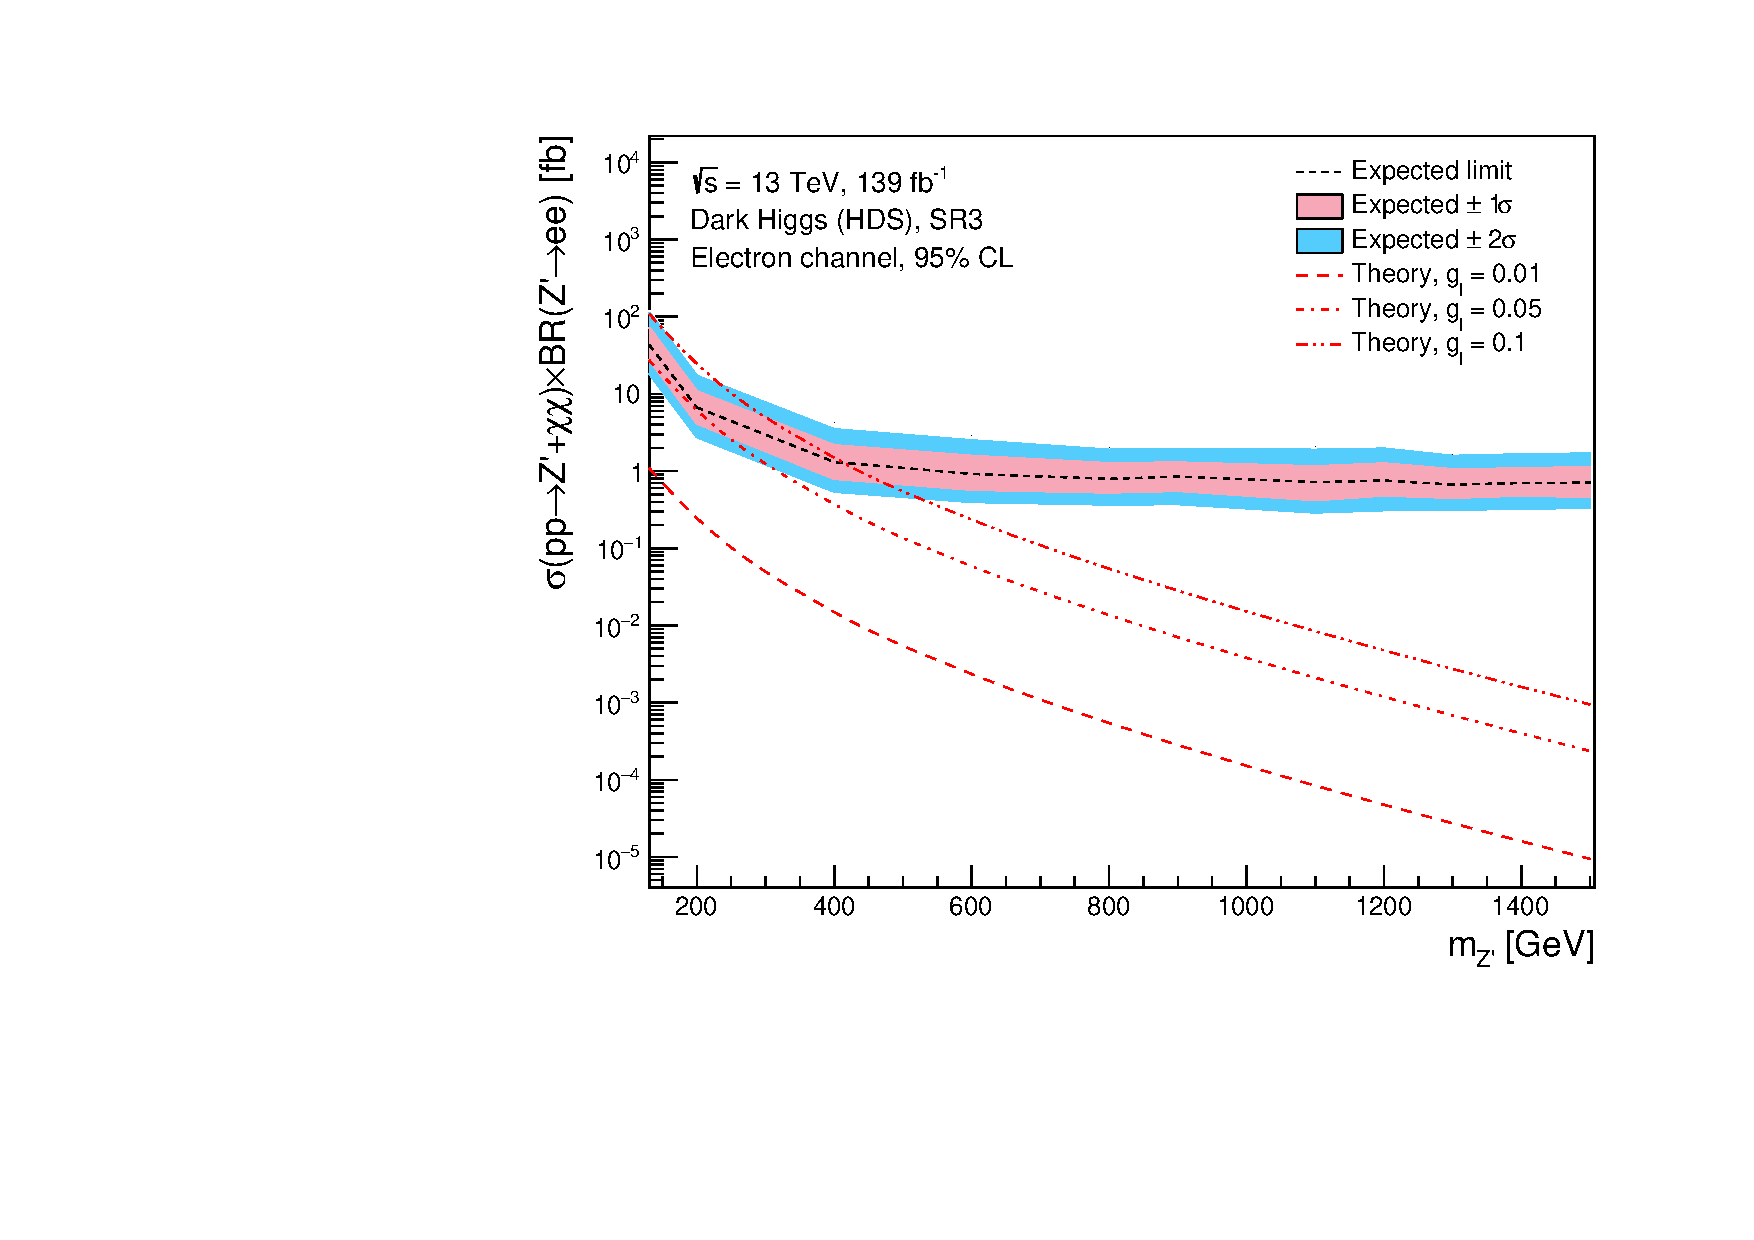
\includegraphics[width=1\textwidth]{Limits/Model_independent/150/DH_HDS/mass_exclusion_ee.pdf}
   \end{subfigure}
   \hfill
   \begin{subfigure}[b]{0.49\textwidth}
      \centering
      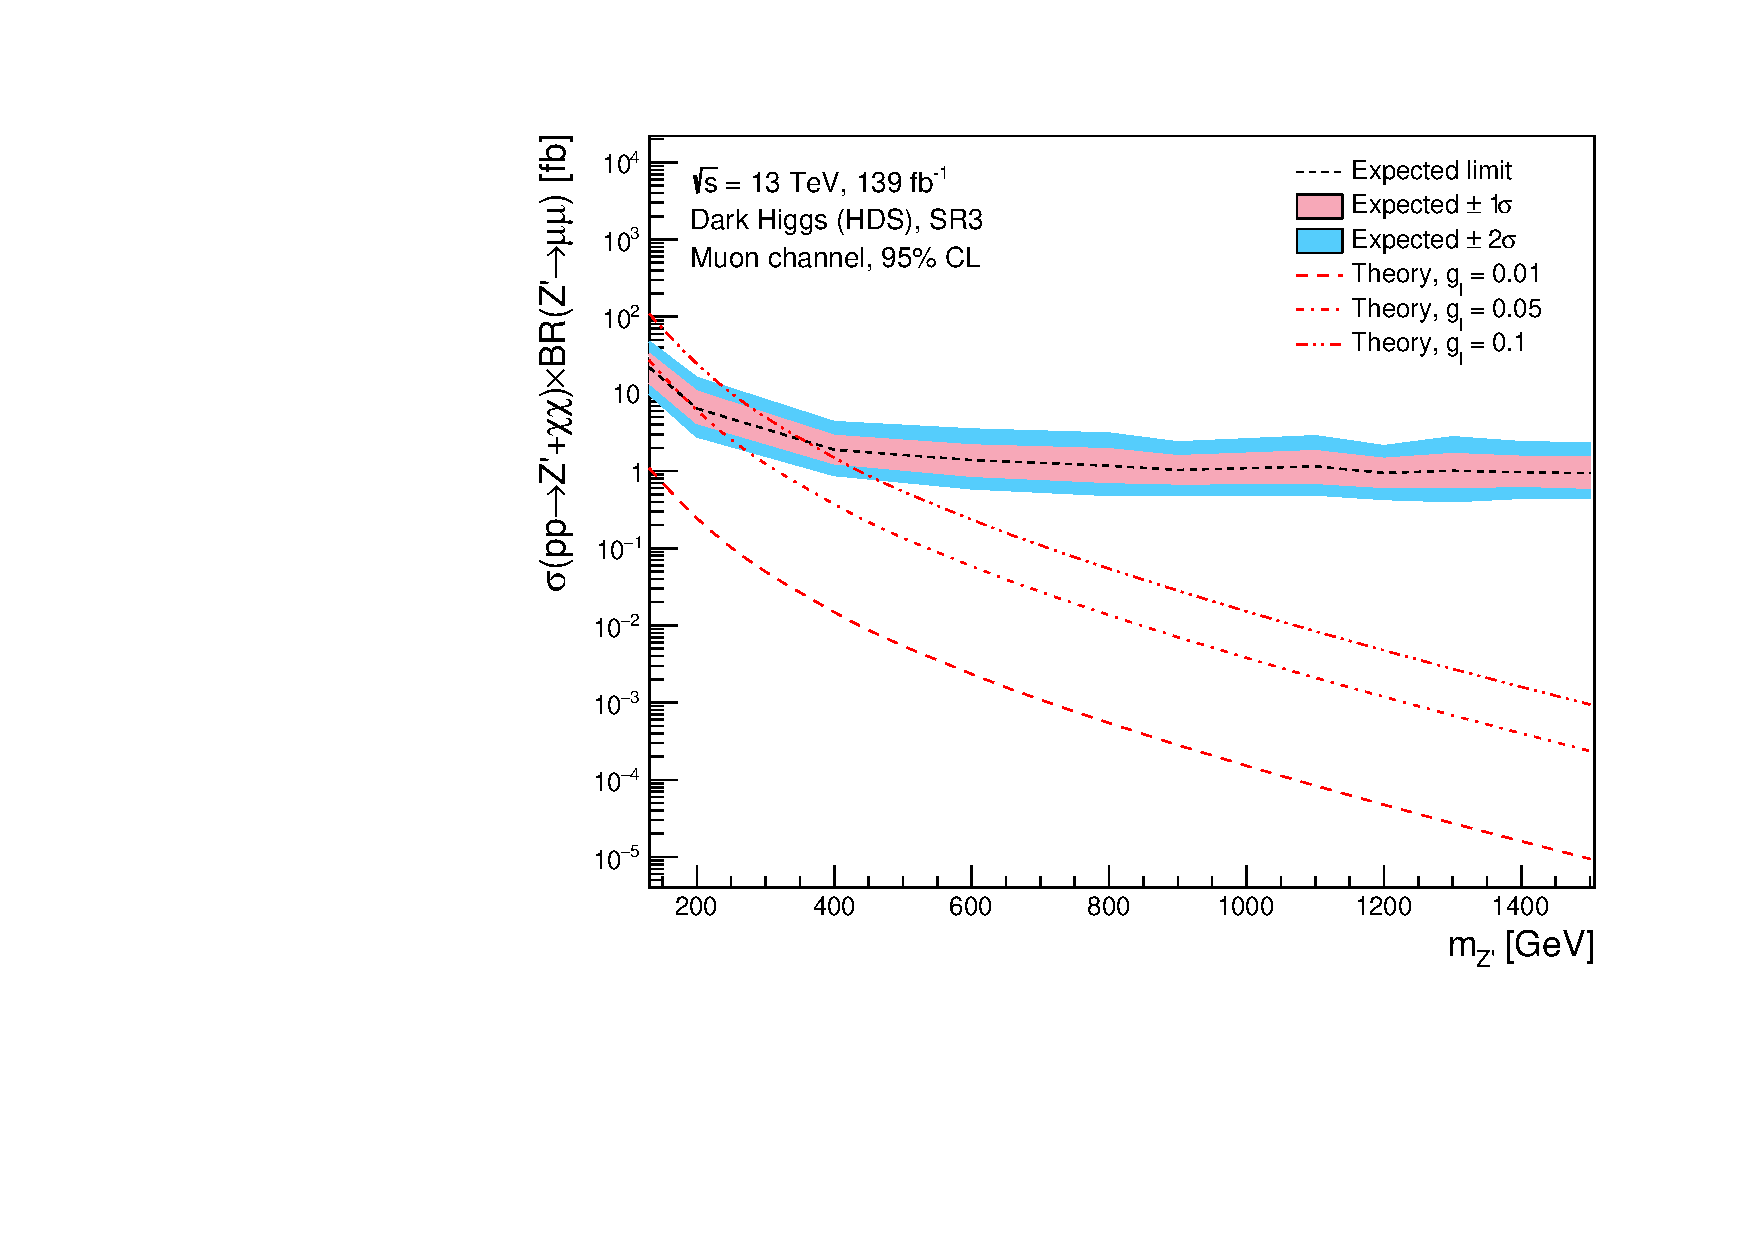
\includegraphics[width=1\textwidth]{Limits/Model_independent/150/DH_HDS/mass_exclusion_uu.pdf}
   \end{subfigure}
   \caption{Mass exclusiion limits results for DH HDS model on $ee$ and $\mu\mu$ channel in all SRs}\label{fig:DH_HDS_me_SRS}
\end{figure}

\begin{figure}[!ht]
	\centering
	\begin{subfigure}[b]{0.49\textwidth}
      \centering
      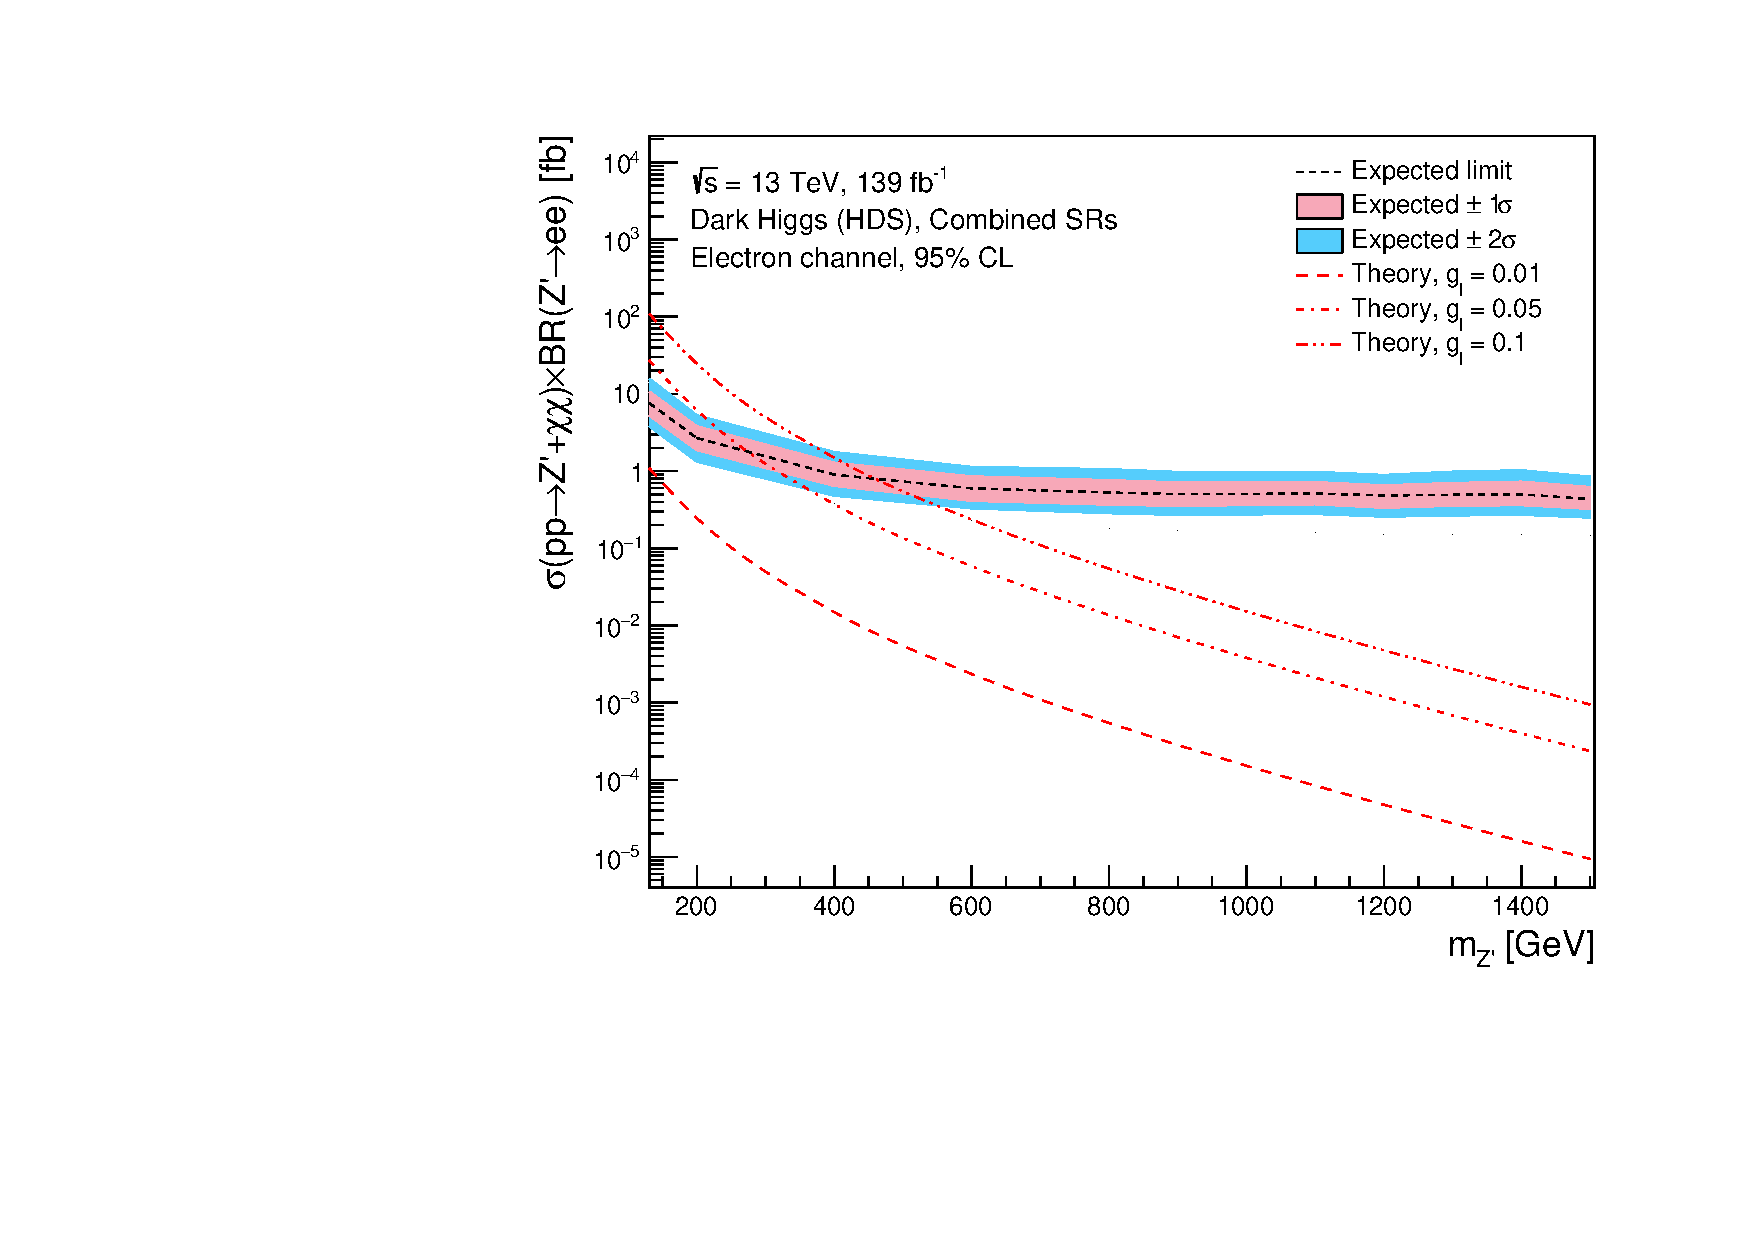
\includegraphics[width=1\textwidth]{Limits/Model_independent/DH_HDS/mass_exclusion_ee.pdf}
   \end{subfigure}
   \hfill
   \begin{subfigure}[b]{0.49\textwidth}
      \centering
      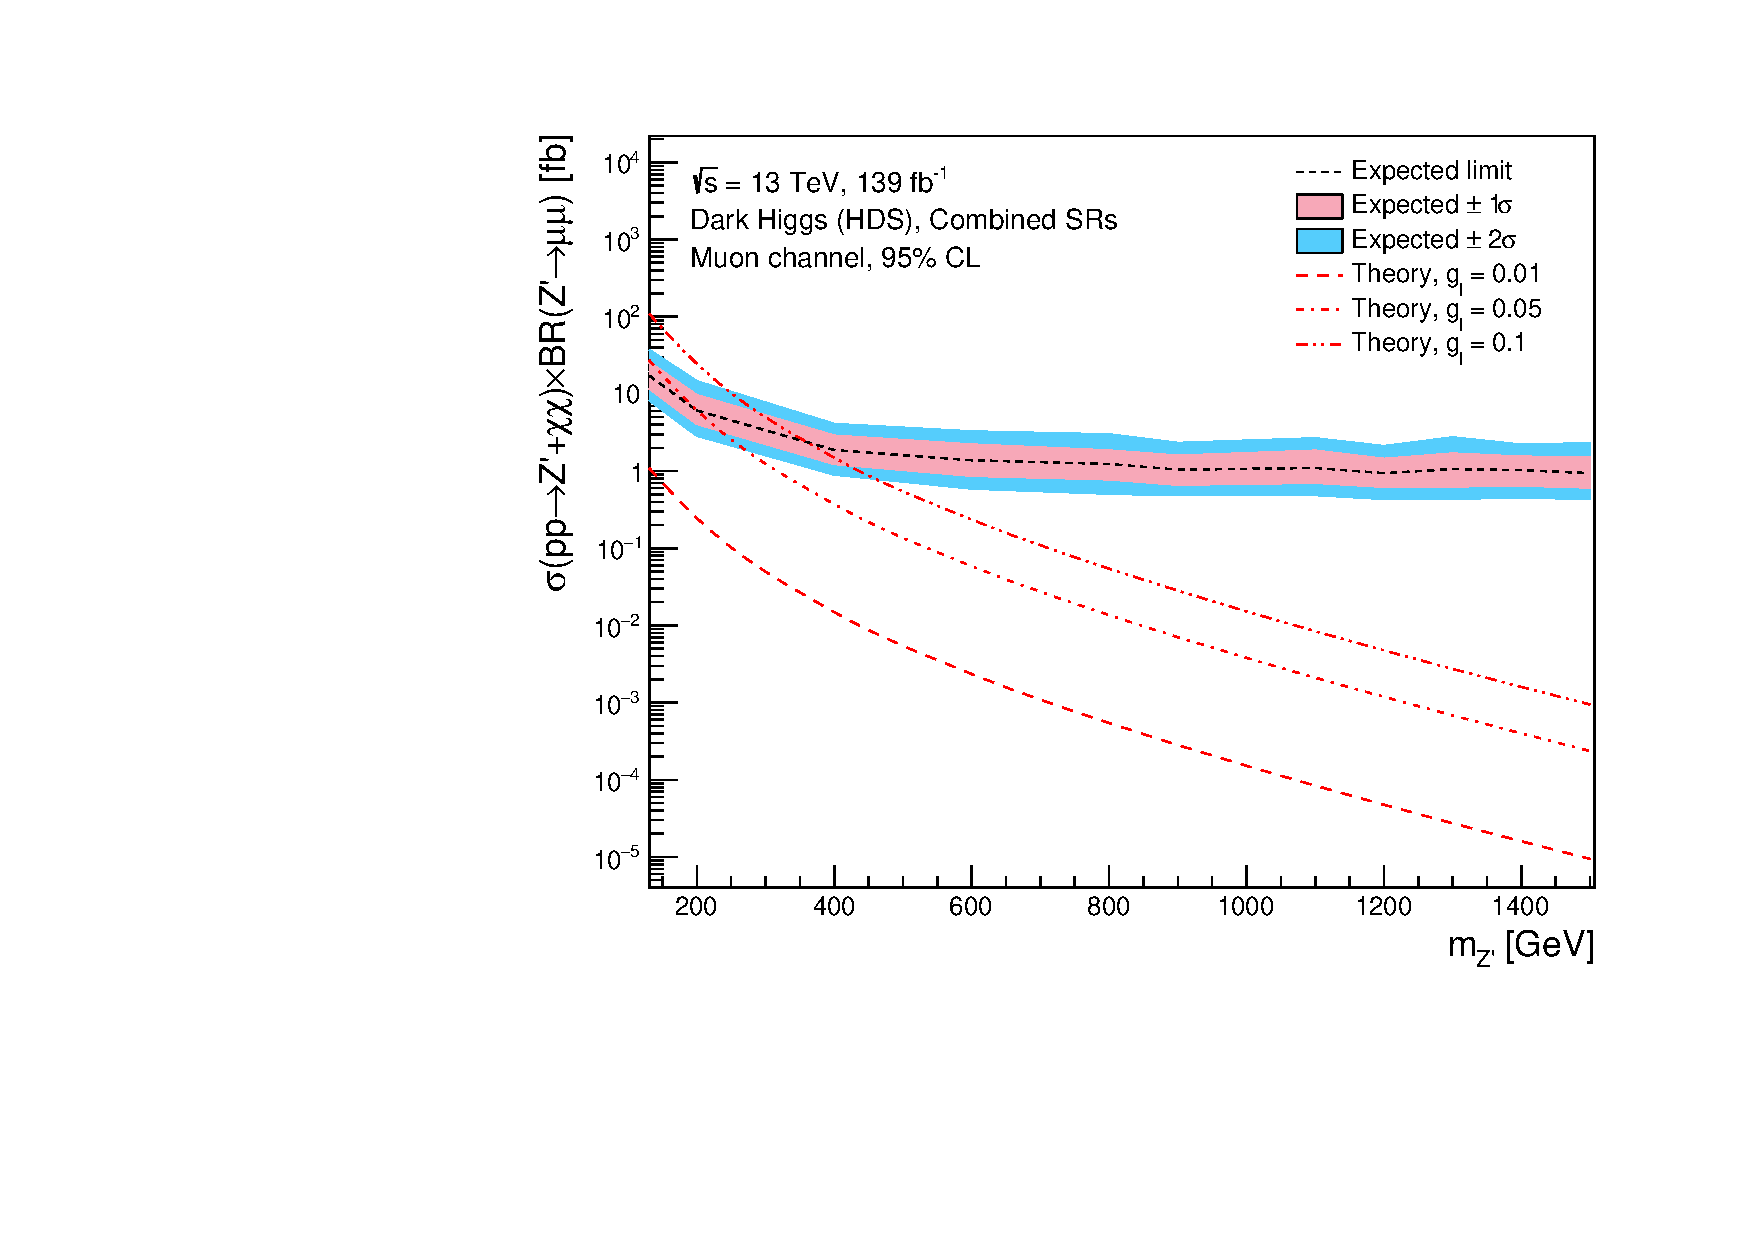
\includegraphics[width=1\textwidth]{Limits/Model_independent/DH_HDS/mass_exclusion_uu.pdf}
   \end{subfigure}
   \caption{Mass exclusiion limits results for DH HDS model on $ee$ and $\mu\mu$ channel in combined SRs}\label{fig:DH_HDS_me_comb}
\end{figure}
\clearpage
\section{Mass exclusion limits for the combined channels}
\begin{figure}[!ht]
	\centering
	\begin{subfigure}[b]{0.49\textwidth}
      \centering
      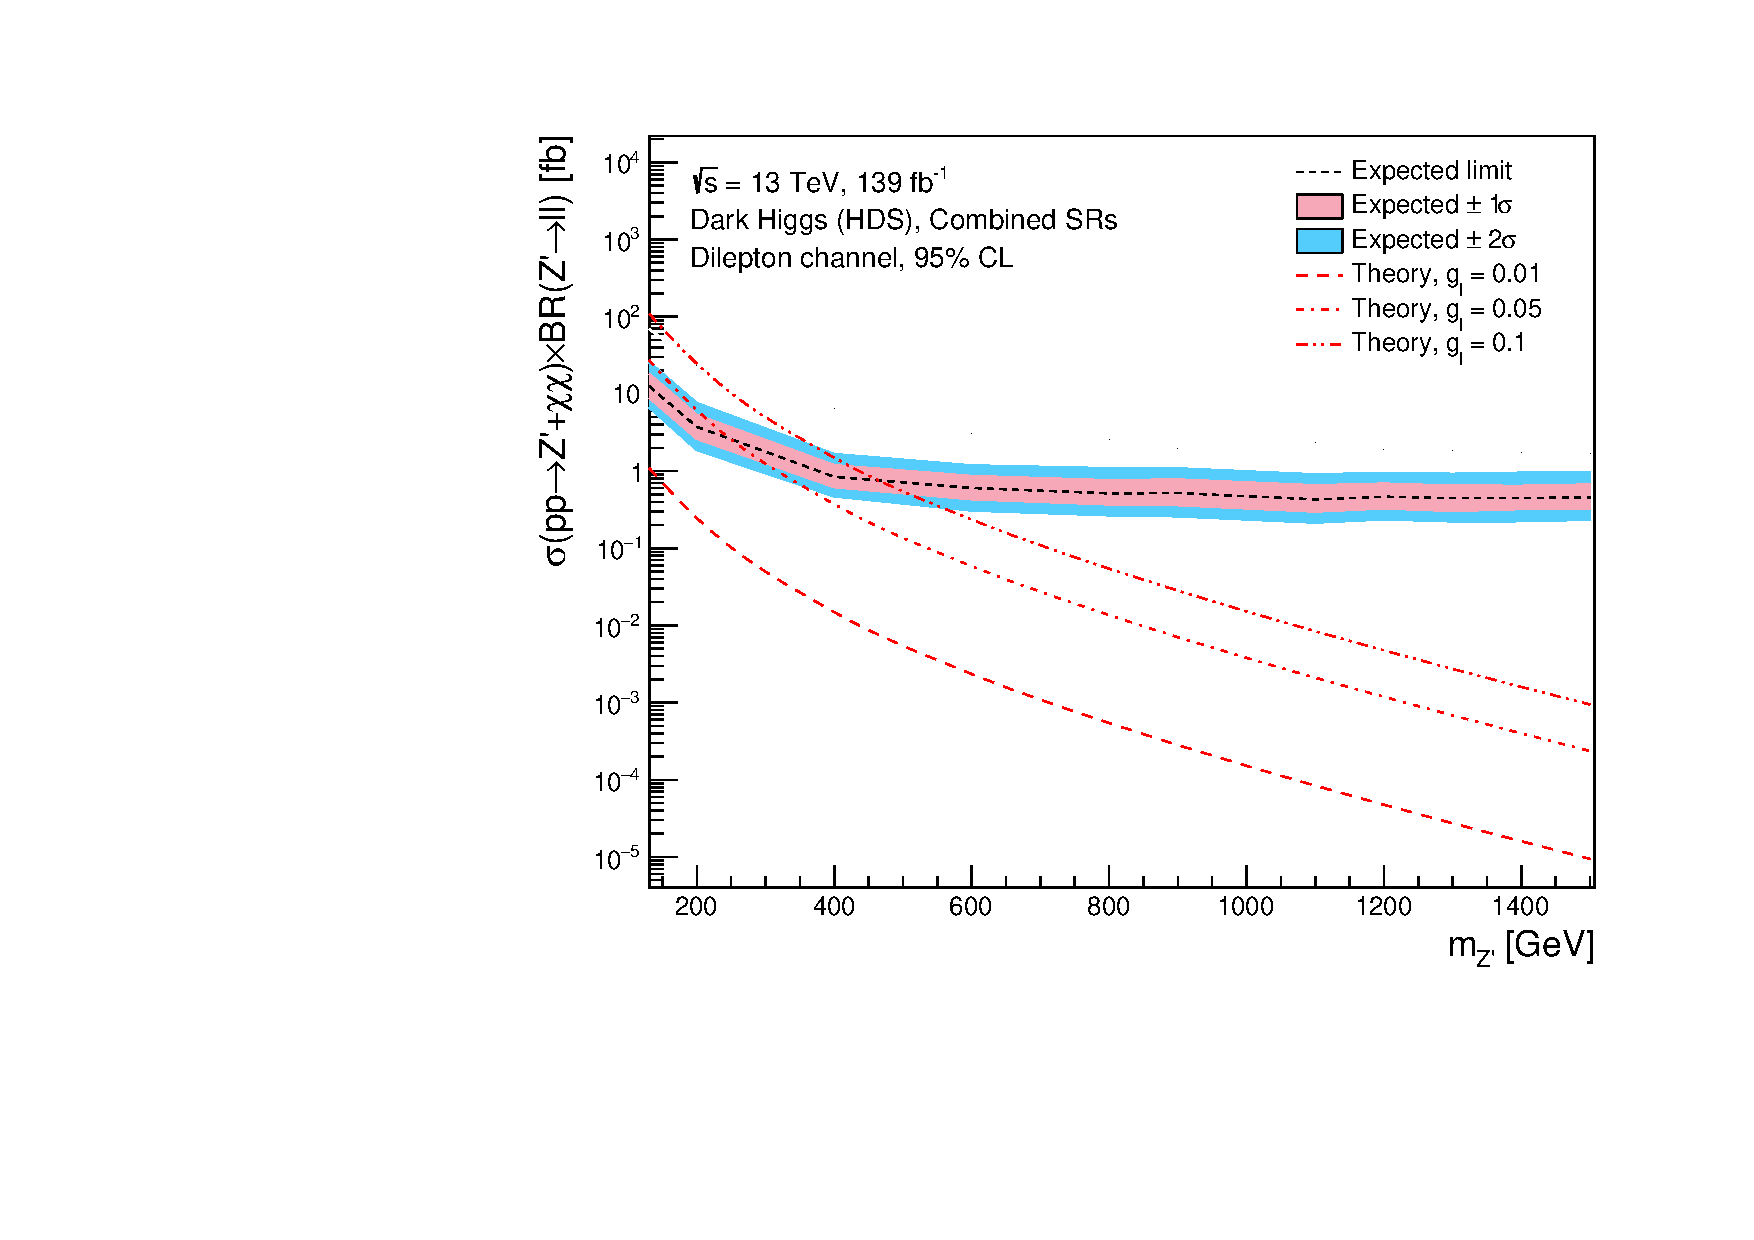
\includegraphics[width=1\textwidth]{Limits/Model_independent/DH_HDS/mass_exclusion_comb.pdf}
      % \caption{When including new variables and using 100 bins}
   \end{subfigure}
   \hfill
   \begin{subfigure}[b]{0.49\textwidth}
      \centering
      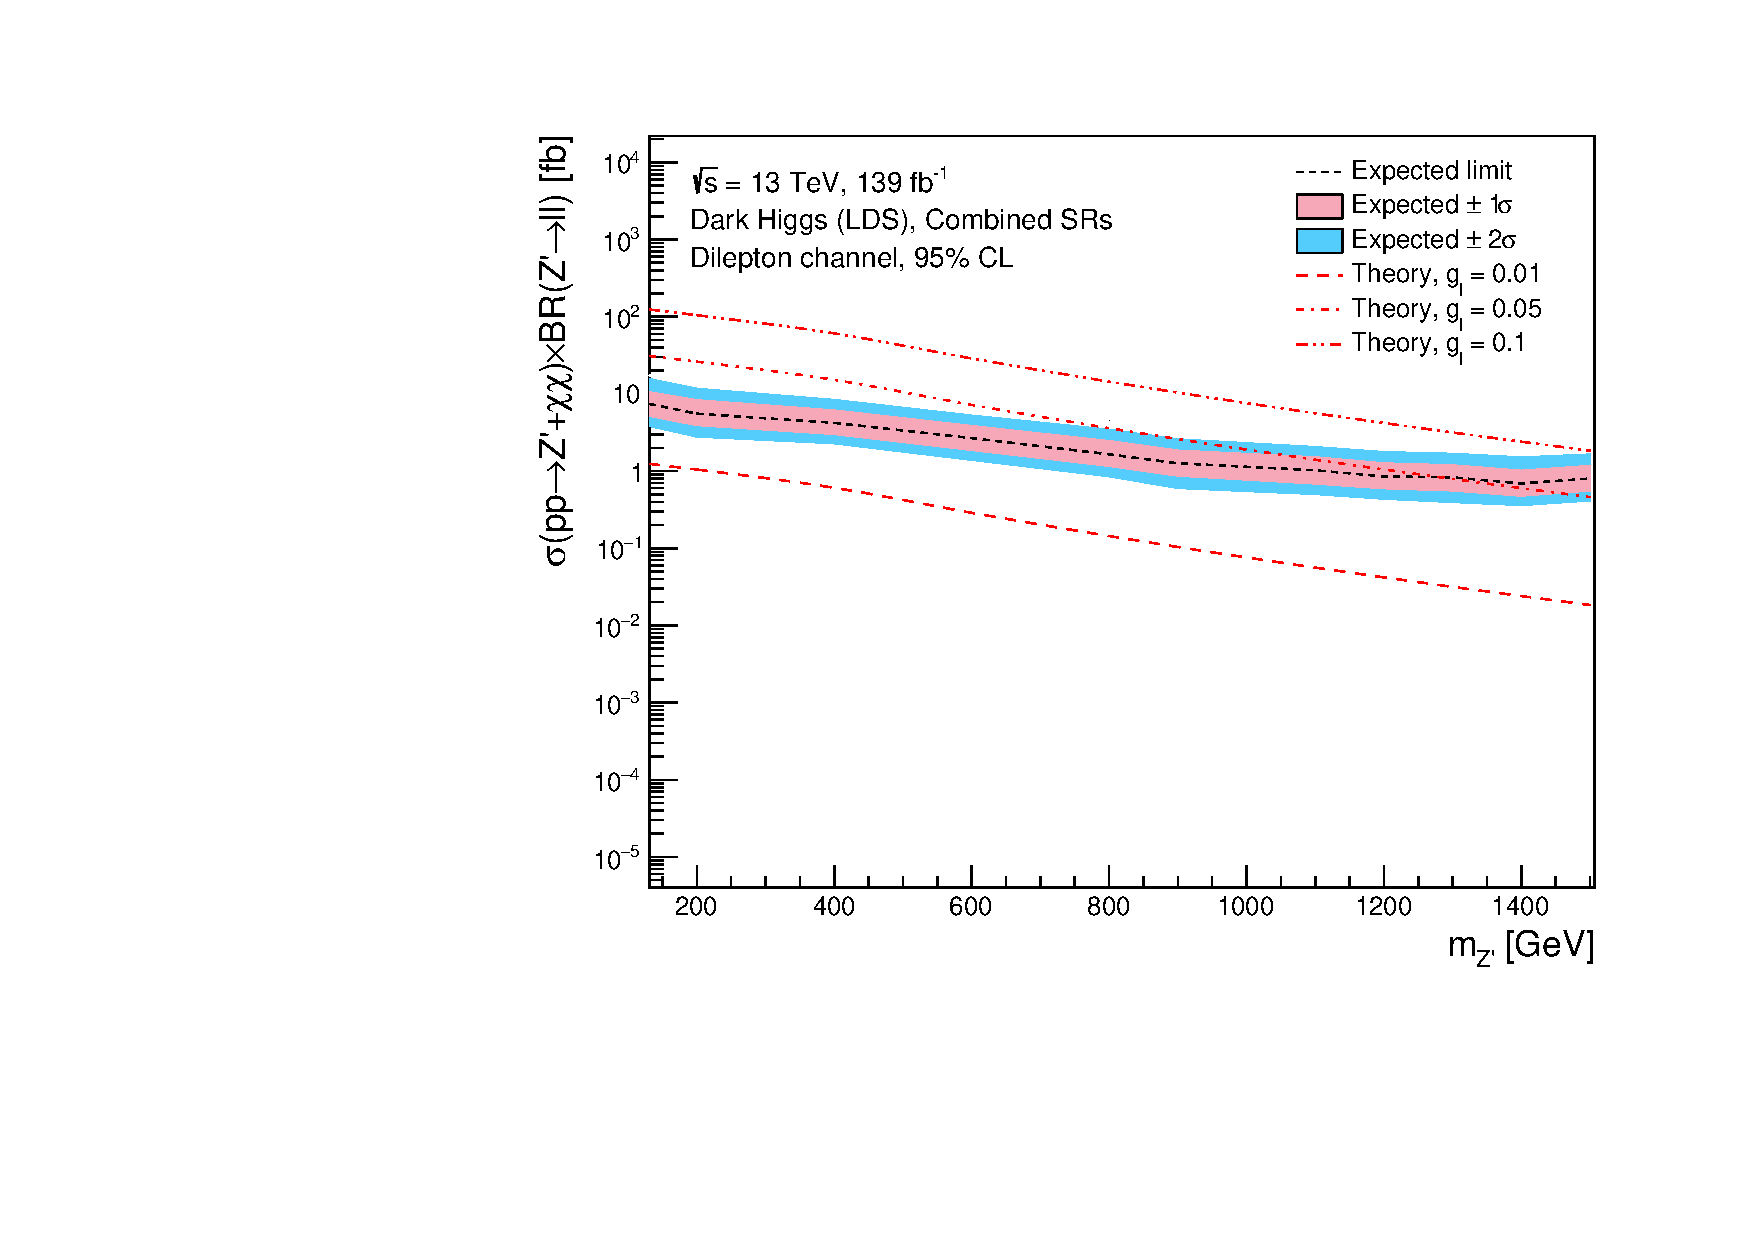
\includegraphics[width=1\textwidth]{Limits/Model_independent/DH_LDS/mass_exclusion_comb.pdf}
      % \caption{Expected significance of a)}
   \end{subfigure}
   \hfill
   \begin{subfigure}[b]{0.49\textwidth}
      \centering
      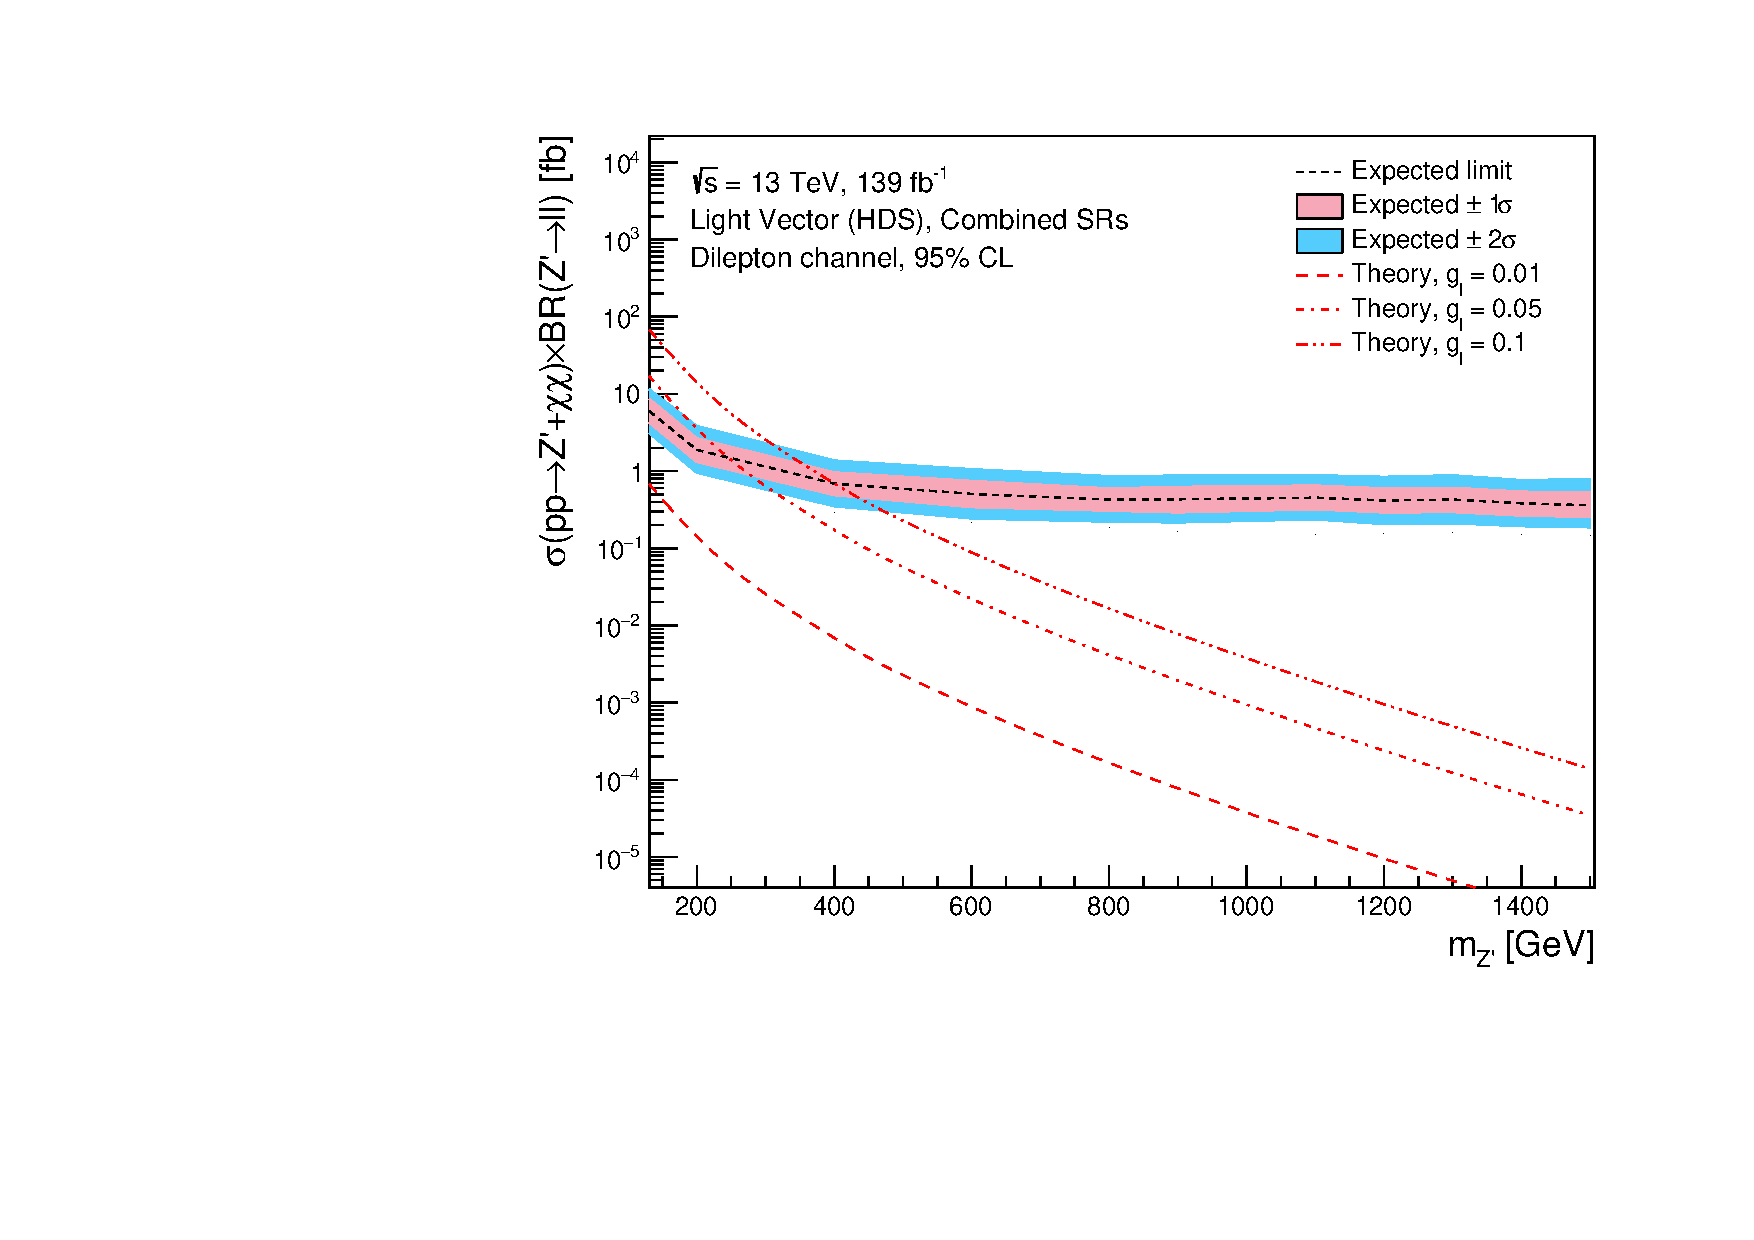
\includegraphics[width=1\textwidth]{Limits/Model_independent/LV_HDS/mass_exclusion_comb.pdf}
      % \caption{When including new variables and using 50 bins}
   \end{subfigure}
   \hfill
   \begin{subfigure}[b]{0.49\textwidth}
      \centering
      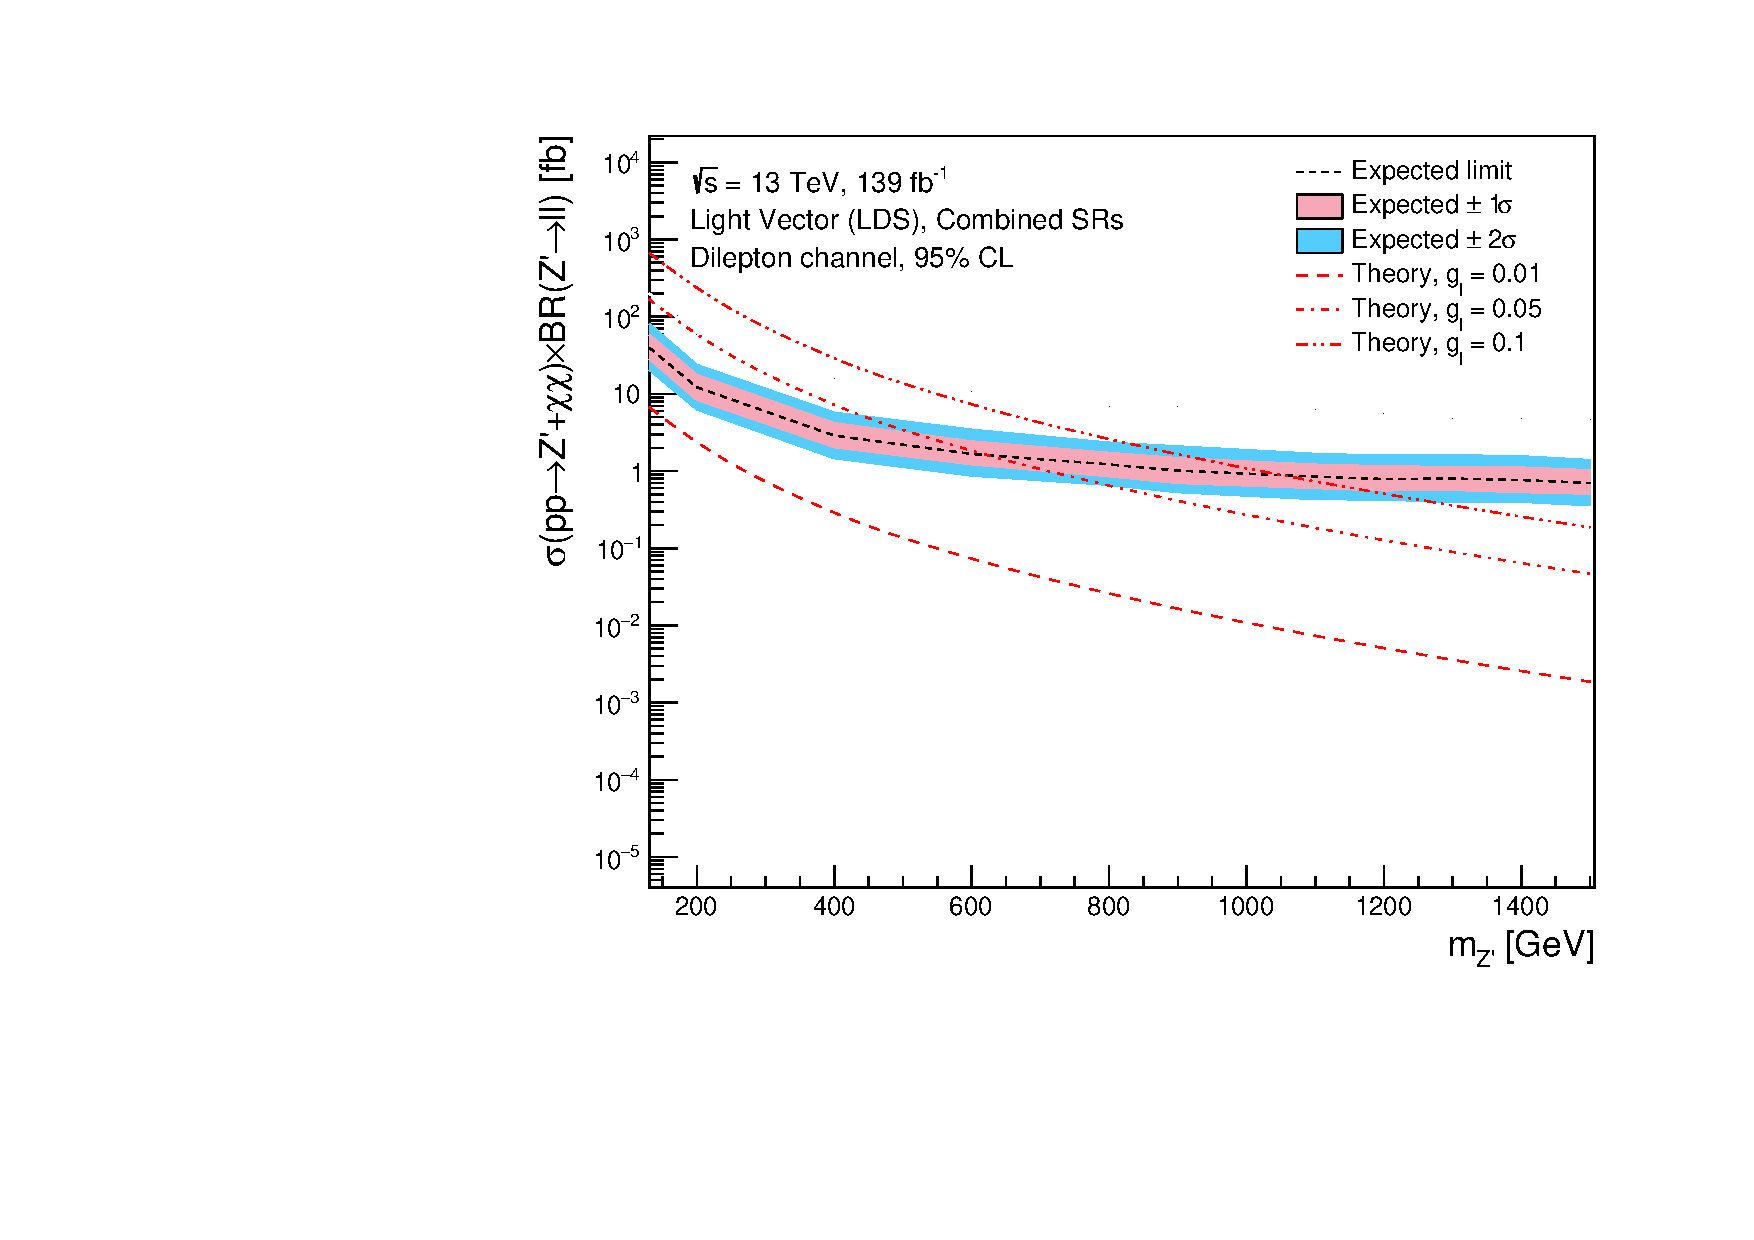
\includegraphics[width=1\textwidth]{Limits/Model_independent/LV_LDS/mass_exclusion_comb.pdf}
      % \caption{Expected significance of c)}
   \end{subfigure}
   \hfill
	\begin{subfigure}[b]{0.49\textwidth}
      \centering
      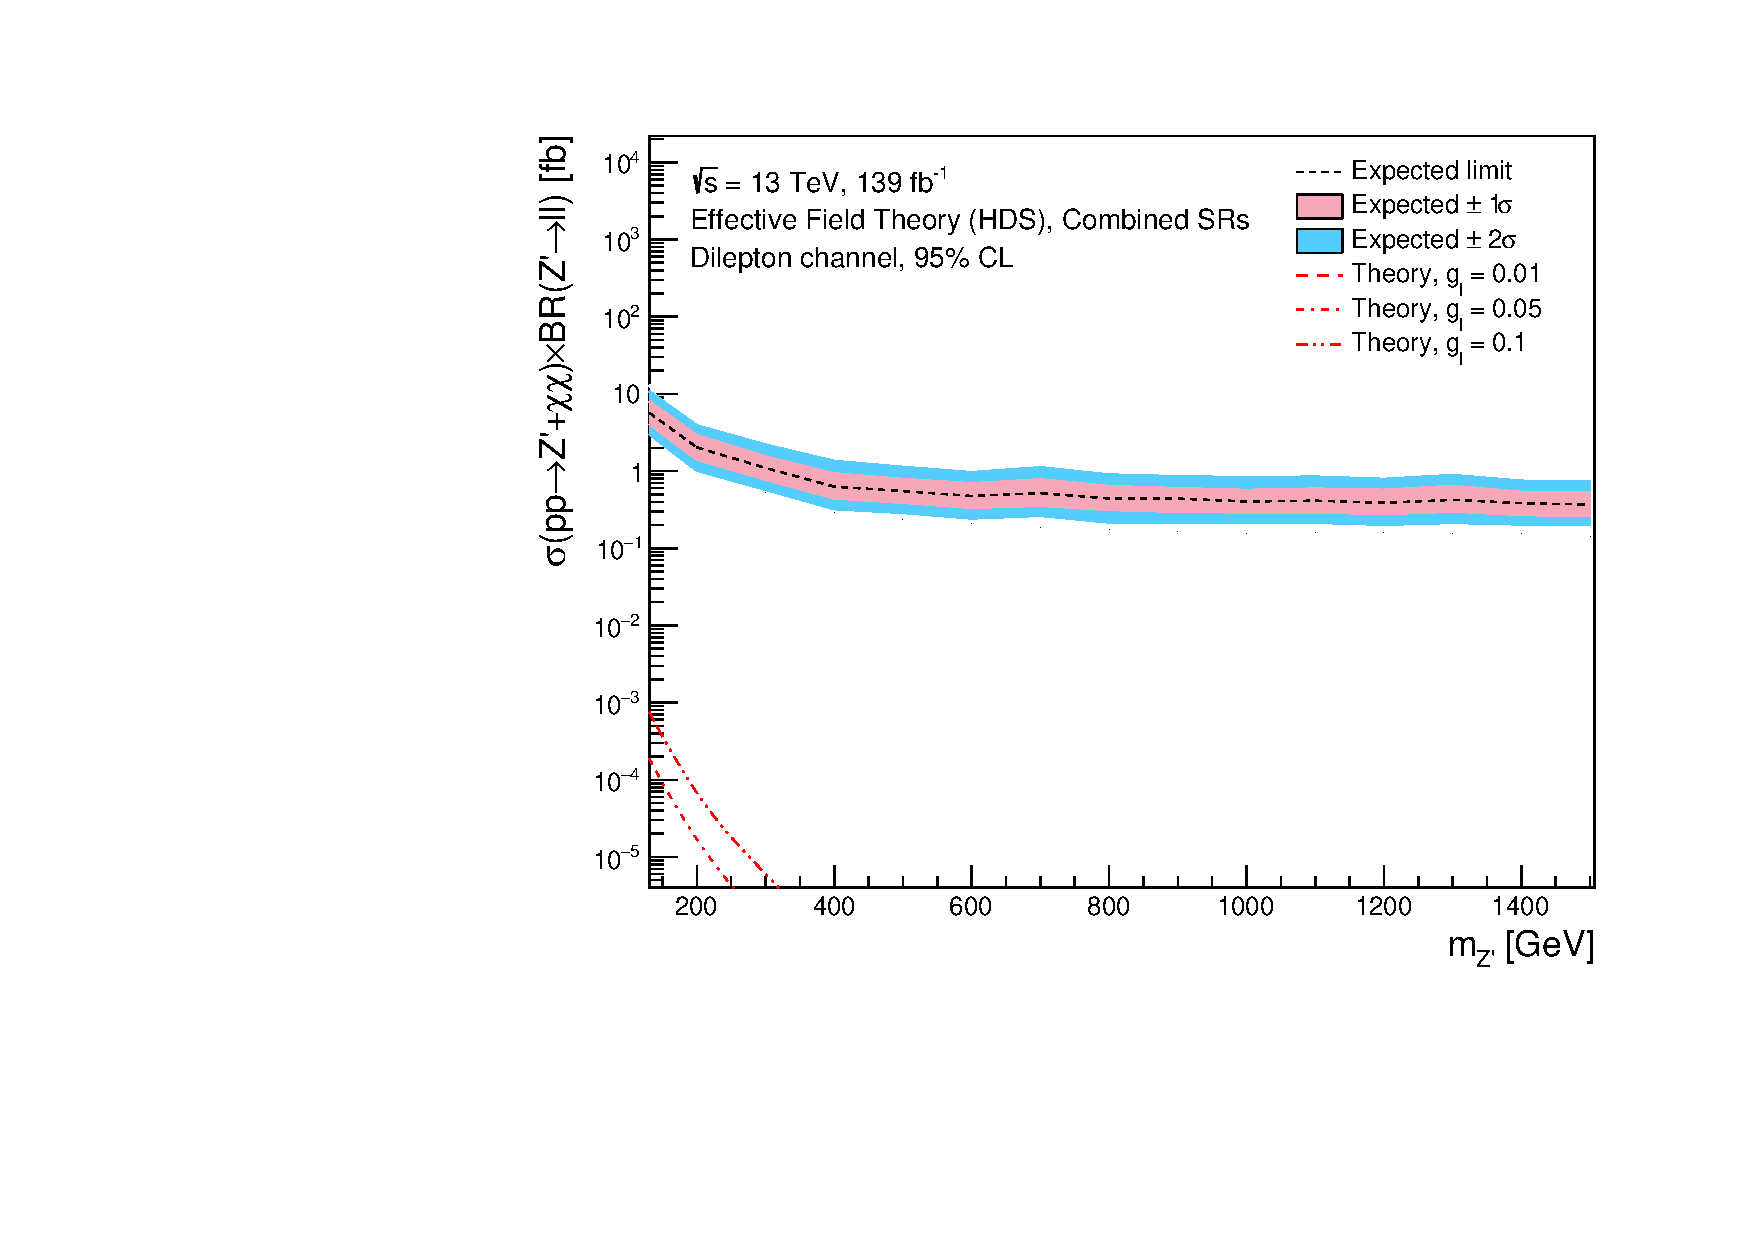
\includegraphics[width=1\textwidth]{Limits/Model_independent/EFT_HDS/mass_exclusion_comb.pdf}
      % \caption{When excluding new variables and using 50 bins}
   \end{subfigure}
   \hfill
   \begin{subfigure}[b]{0.49\textwidth}
      \centering
      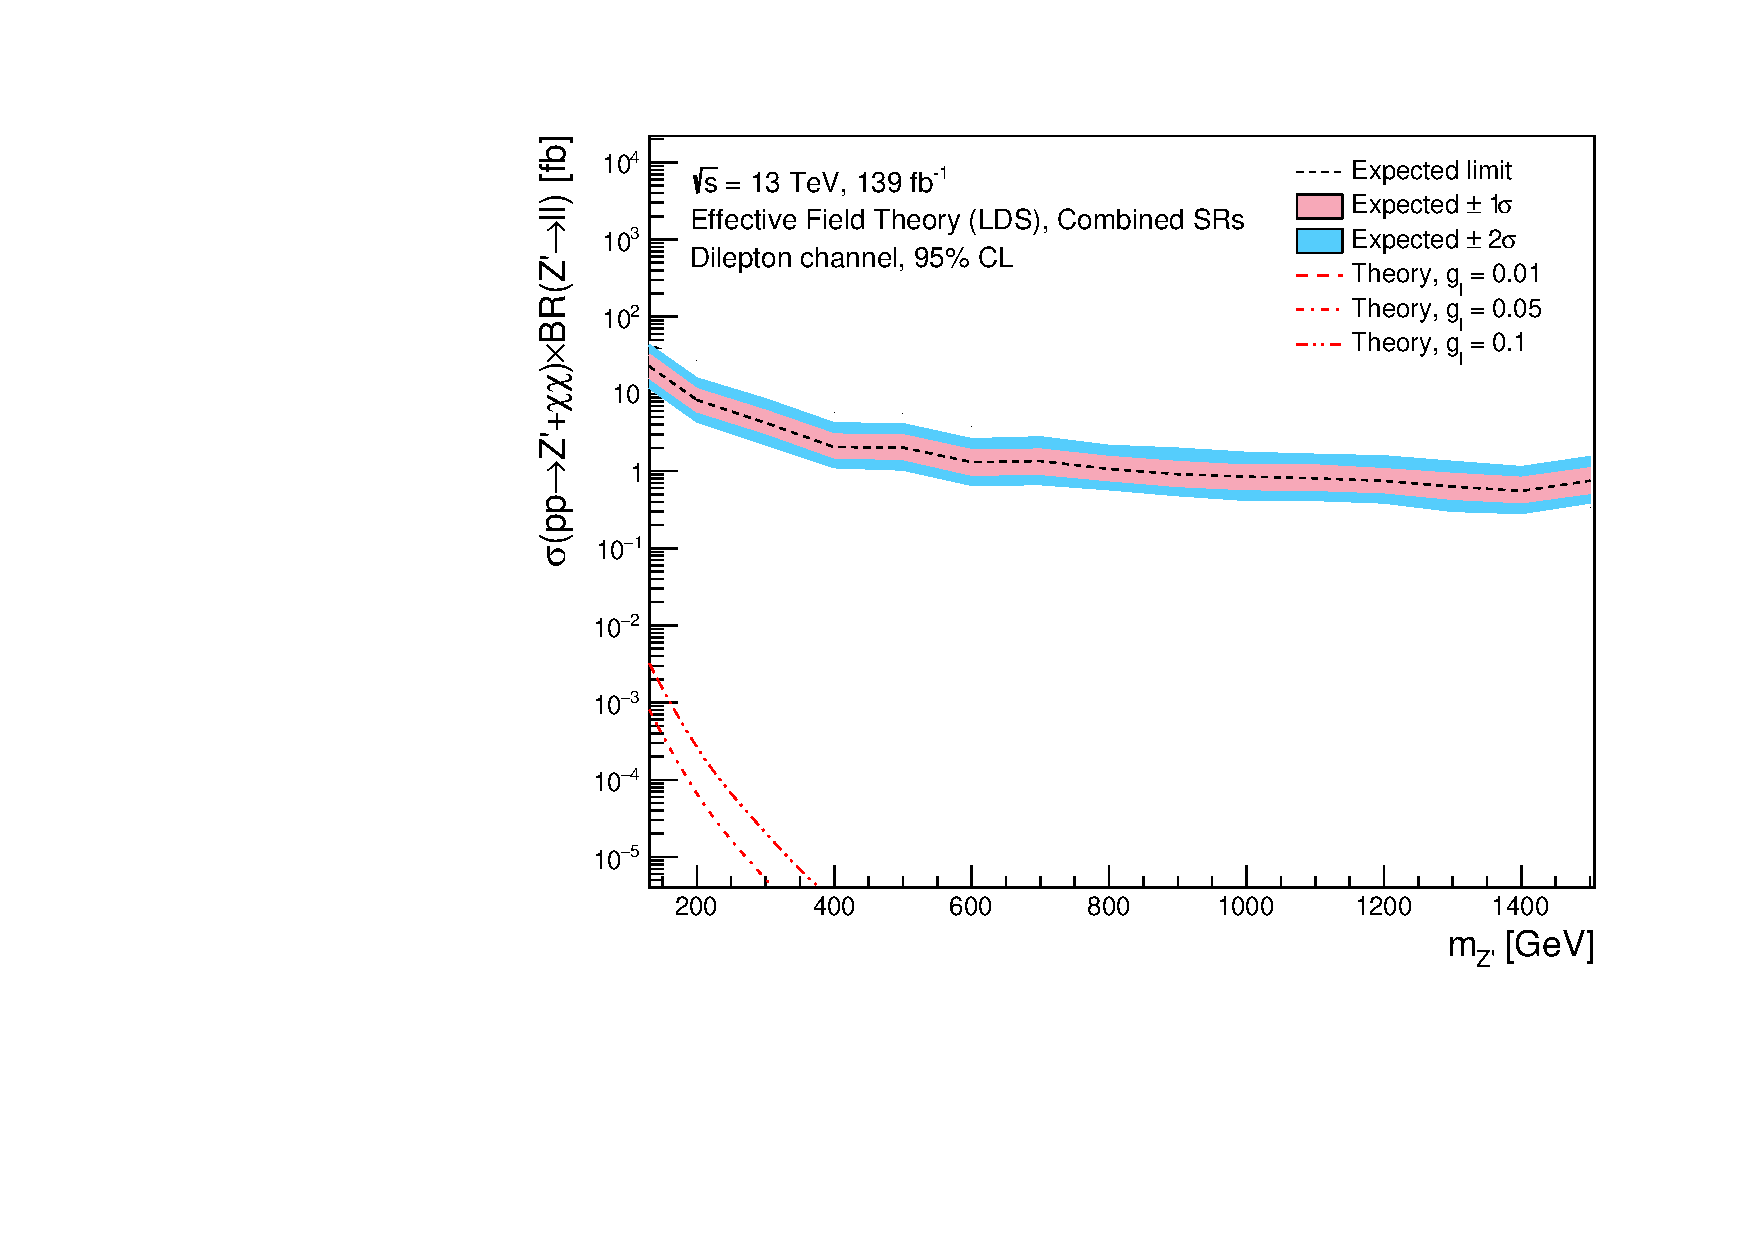
\includegraphics[width=1\textwidth]{Limits/Model_independent/EFT_LDS/mass_exclusion_comb.pdf}
      % \caption{Expected significance of e)}
   \end{subfigure}
   \caption[Mass exclusion limits of combined $ee$ and $\mu\mu$ channel for all models]{Mass exclusion limits of combined $ee$ and $\mu\mu$ channel for all models}\label{fig:model_dep_exclusions}
\end{figure}
\clearpage

\end{document}